\documentclass[11pt,twoside]{article}
\addtolength{\textwidth}{0.5in}
\usepackage{epsfig,amsfonts,color}
\usepackage{amsmath}
\bibliographystyle{plain}
\usepackage{amssymb, palatino, geometry,url}
\usepackage{algorithmic}
\usepackage[noresetcount,lined,boxed]{algorithm2e} % ... for algorithms
\usepackage[colorlinks=true,linkcolor=blue,citecolor=blue,urlcolor=blue]{hyperref}
\geometry{letterpaper,
          left       = 0.9in,
          right      = 0.9in,
          top        = 0.9in,
          bottom     = 0.9in}
\linespread{1.2}

\usepackage{fancyhdr}
\usepackage{enumerate}
\usepackage{float}
\usepackage{subcaption}
\usepackage{graphicx}
\usepackage{caption}
\newcommand{\twopart}[4]
{
	\left\{
		\begin{array}{ll}
			#1 & \mbox{ } {\textrm{#2}} \\
			#3 & \mbox{ } {\textrm{#4}}
		\end{array}
	\right.
}

\newcommand{\N}{\mathbb{N}}
\newcommand{\Z}{\mathbb{Z}}
\newcommand{\Q}{\mathbb{Q}}
\newcommand{\R}{\mathbb{R}}
\usepackage{placeins}
\usepackage{lineno}
%\linenumbers
\usepackage{array}
\newcolumntype{L}[1]{>{\raggedright\let\newline\\\arraybackslash\hspace{0pt}}m{#1}}
\newcolumntype{C}[1]{>{\centering\let\newline\\\arraybackslash\hspace{0pt}}m{#1}}
\newcolumntype{R}[1]{>{\raggedleft\let\newline\\\arraybackslash\hspace{0pt}}m{#1}}
\usepackage{graphicx}

\begin{document}

\title{Analysis of Multi-Scale Energy Markets using Stochatic Optimization Techniques}

\author{\textbf{\textit{ISyE 719 Course Project}}\\ \\Apoorva Sampat and Ranjeet Kumar\\
 {\small Department of Chemical and Biological Engineering}\\
 {\small \;University of Wisconsin, 1415 Engineering Dr, Madison, WI 53706, USA}}
\date{}
\maketitle

\begin{abstract}
Electricity markets operate at multiple timescales (from hours to milliseconds) to ensure that supply and demands are matched in real time. These markets involve uncertainties because future electricity prices and demands are unknown at the time of decision-making, e.g. energy sale and purchase commitments by generators. We use stochastic programming techniques to study flexibility and economic opportunities provided by a battery in these markets, namely day-ahead (1-hour timescale) and real-time (5-minute timescale) markets. In this work we consider uncertainty only in electricity loads and determine optimal participation strategies using methods like receding horizon scheme, dual dynamic programming and *fullproblem (scenario sampling)*. We also determine bounds on expected policy costs by using perfect information and two-stage approximation (with restriction on states). We compare the costs of participation in exclusively in day-ahead market and both day-ahead and real-time markets. Our results show that market participation only in day-ahead energy markets can *significantly* reduce economic flexibility as compared to participating in both levels of markets.
\end{abstract}


\section{Introduction}
A diverse set of energy systems such as generators, batteries, wind turbines and flywheels can participate in electricity markets. This participation is governed by rules set by ISOs (Independent System Operators) such as California ISO, PJM (Pennsylvania-New Jersey-Maryland) Interconnection and Midcontinent ISO, under whose jurisdiction the market falls. The markets are structured at multiple time levels, namely day ahead (hourly market commitments) and real time markets (commitments ranging from minutes to seconds). In day-ahead markets the electricity is traded in intervals of 1 hour with the prices being constant in each interval of 1 hour and varying with intervals. Real time markets, on the other hand can have varying time scales depending on the ISO operating it. The real-lime market is a spot market in which utilities can buy power to meet the last few increments of demand not covered in their day ahead schedules. It is also the market that secures energy reserves, held ready and available for ISO use if needed, and the energy needed to regulate transmission line stability \footnote{http://www.caiso.com/market/Pages/MarketProcesses.aspx}.The frequency of energy price variation is different for day-ahead and real time markets (Figure \ref{eprices}). The real time market is more volatile, and at times the prices can even go negative here. This provides an opportunity to the building-battery system to buy electricity at negative price and meet its load demands. The fast dynamics of battery helps it to capture these spikes in prices and maximize its revenue potential. 

\begin{figure}[h!tp]
\centering
\begin{subfigure}[b]{0.32\textwidth} 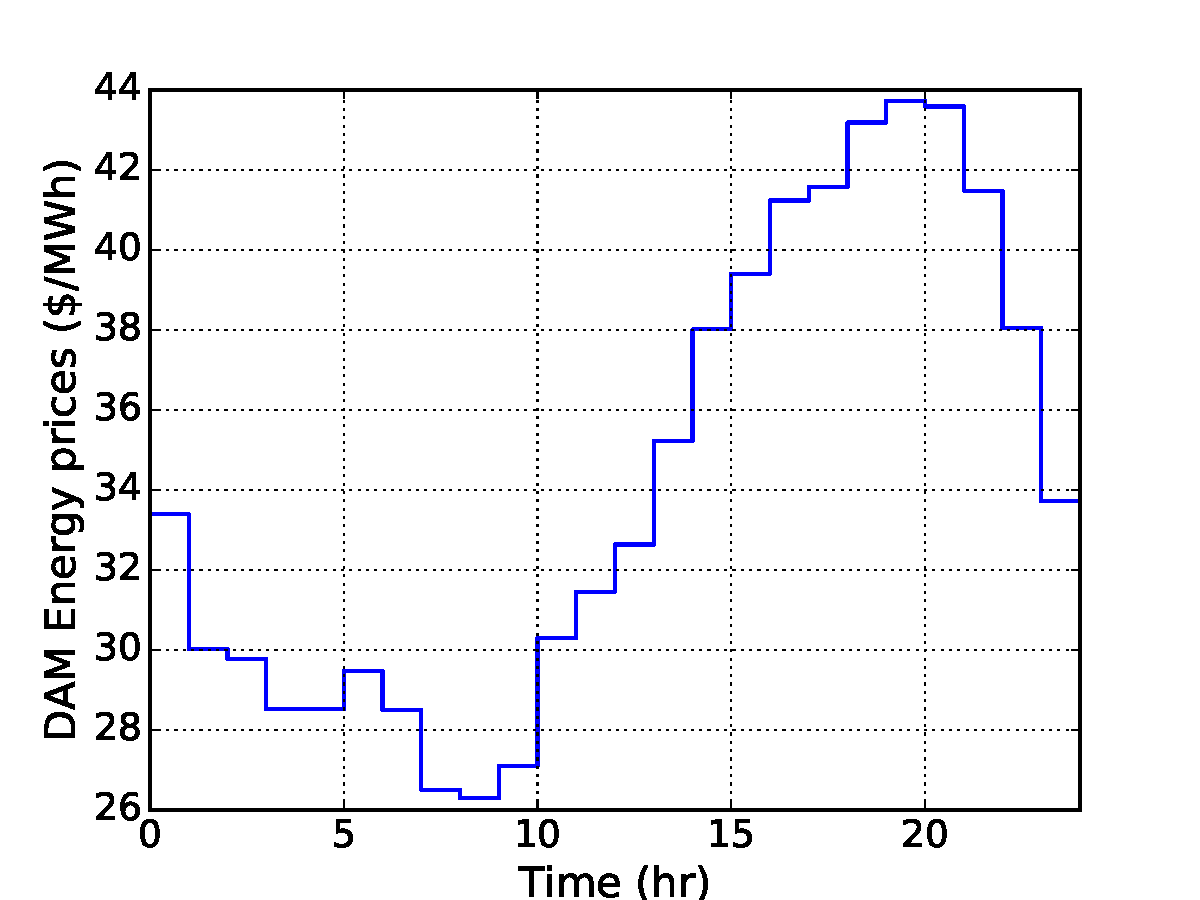
\includegraphics[width=\textwidth]{Figures/damprices.pdf} \caption{Day-ahead market}\label{damprices} \end{subfigure} \hfill
\begin{subfigure}[b]{0.32\textwidth} 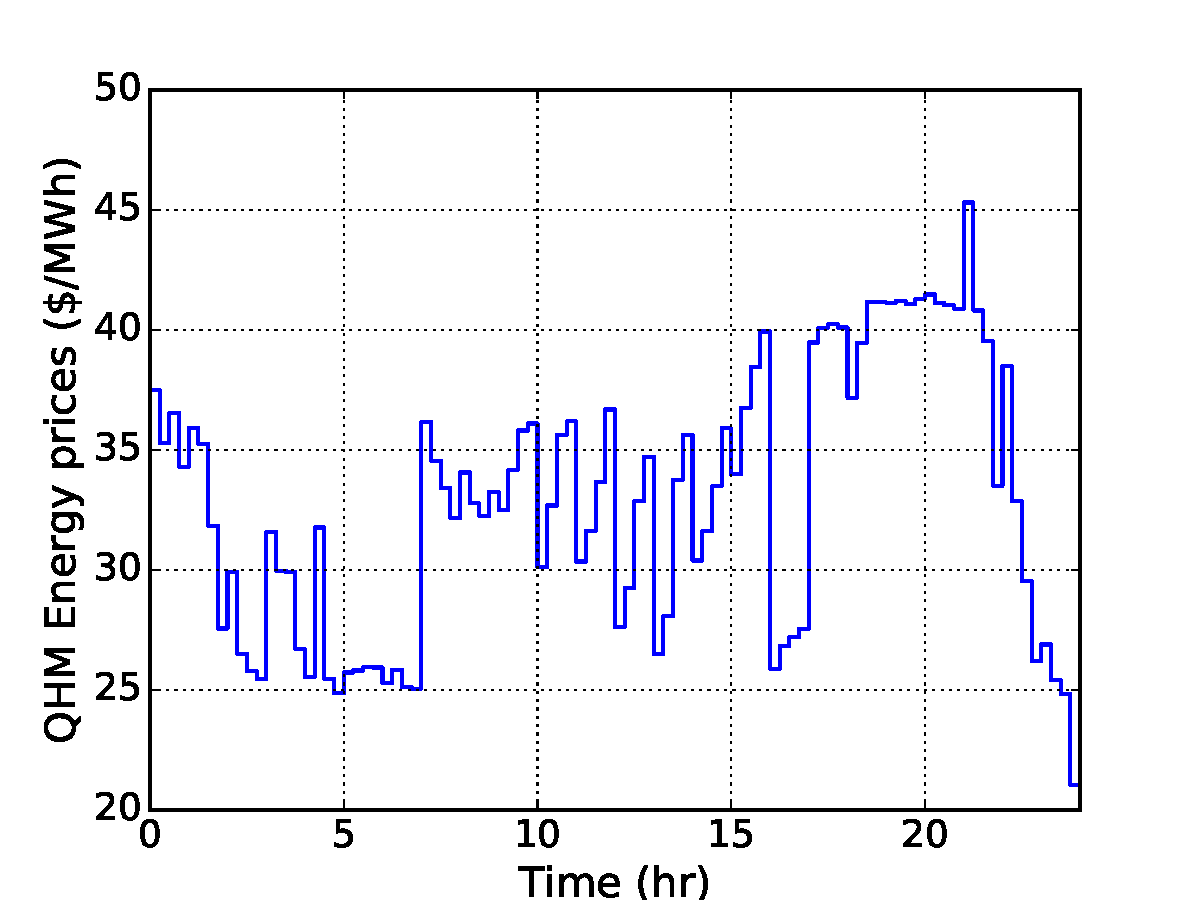
\includegraphics[width=\textwidth]{Figures/qhmprices.pdf} \caption{Quarter-hourly market}\label{qhmprices} \end{subfigure} \hfill
\begin{subfigure}[b]{0.32\textwidth} 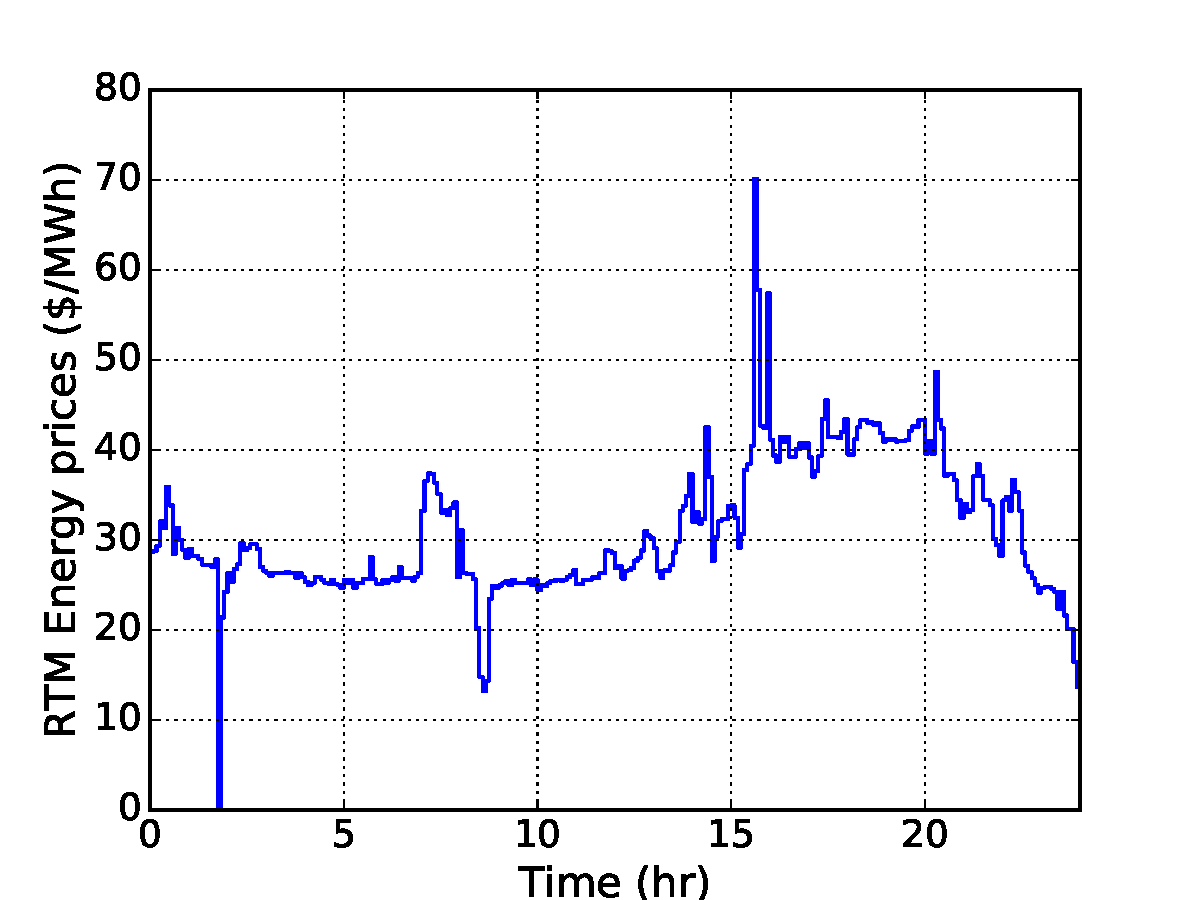
\includegraphics[width=\textwidth]{Figures/rtmprices.pdf} \caption{Real-time market}\label{rtmprices}\end{subfigure} \hfill
\caption{Energy prices for one day in the markets in California}\label{eprices}
\end{figure}

Apart from price variations, the introduction of more renewable power sources in the grid such as wind and solar energy, there are greater variations and uncertainties in the net load as well. Since these sources depend on intermittent conditions such as weather, they introduce slow dynamics to the grid. Thus systems with faster dynamic responses such as battery and building systems are becoming increasingly important to balance these fluctuations and provide dynamic flexibility to the power grid. Also, factors such as transmission losses, generation cost and congestion affect the value of products (energy, regulation, spinning , non-spinning reserves) offered at different timescales. These fluctuations being inherently uncertain, determining the optimal participation policy requires analysis using stochastic optimization techniques.
\section{Problem Definition and Decision-Making Setting}\label{sec:setting}
We consider a rechargeable Li-ion battery with a building that is inter-connected to the power grid for providing electricity services. Electricity services imply that batteries can provide power to or draw power from the grid. In our current setting, we do not consider participation in regulation or other ancillary services. The operator of the power grid (ISO) compensates the battery-owners for the electricity services provided. The goal for the battery-owners is to maximize the revenues generated by providing services to the grid and at the same time meeting the load demands from building. We consider battery and building as one system (building-battery system) and any unmet load demand from the building is penalized with the corresponding electricity price in real time market.\\
\begin{figure}[h!]
\begin{center}
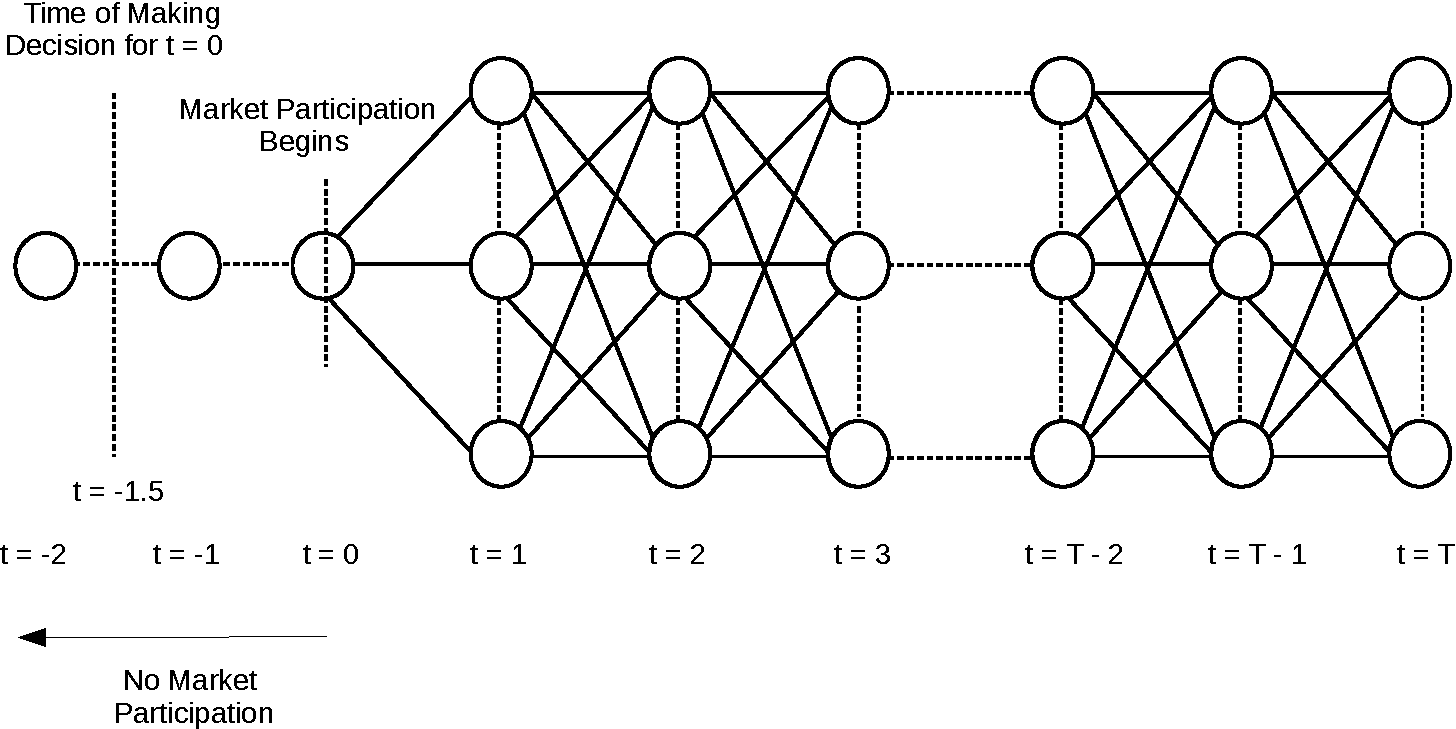
\includegraphics[width=4in]{Figures/scenario_tree-crop.pdf} \caption{Scenario tree at the beginning of market participation}\label{fig:scenario_tree}\end{center}
\end{figure}
We generate a compact scenario tree consisting of 12 sub-intervals between any two hours. One scenario represents a load profile in these 12 subintervals. The participation in market begins at time t = 0 hrs (Figure \ref{fig:scenario_tree}) and decisions can be made latest till 1.5 hrs before any hour (according to market rules set by ISO). Thus our decision making starts at -1.5 hrs (as shown in Figure \ref{fig:scenario_tree}) and our participation begins at t = 0 hrs.   

We divide an annual dataset for electricity loads (available over 5-minute intervals) into 52 subsets of weekly load profiles, i.e 2016 intervals of 5-minute each. This division of data helps in capturing the different load profiles over the weekdays and the weekend. We then use these 52 weekly profiles to generate sample scenarios for our computational experiments (Section \ref{sec:exp}). Since the loads are correlated between time intervals, we formulate a multivariate normal distribution for weekly loads using a mean vector and a covariance matrix. The mean vector (of size 2016 x 1) is the mean of the 52 datasets, but the covariance matrix (of size 2016 x 2016) calculated directly from the 52 datasets cannot be used, since its rank can at most be 52. So we use the Ledoit-Wolf Covariance Estimator \cite{ledoit2004well} (to tackle rank deficiency) for estimating a full rank covariance matrix. We generate 50 samples of load profiles (Figure \ref{fig:loads_scenarios}) for a week using the mean and covariance matrix obtained. 
\begin{figure}[h!]
\begin{center}
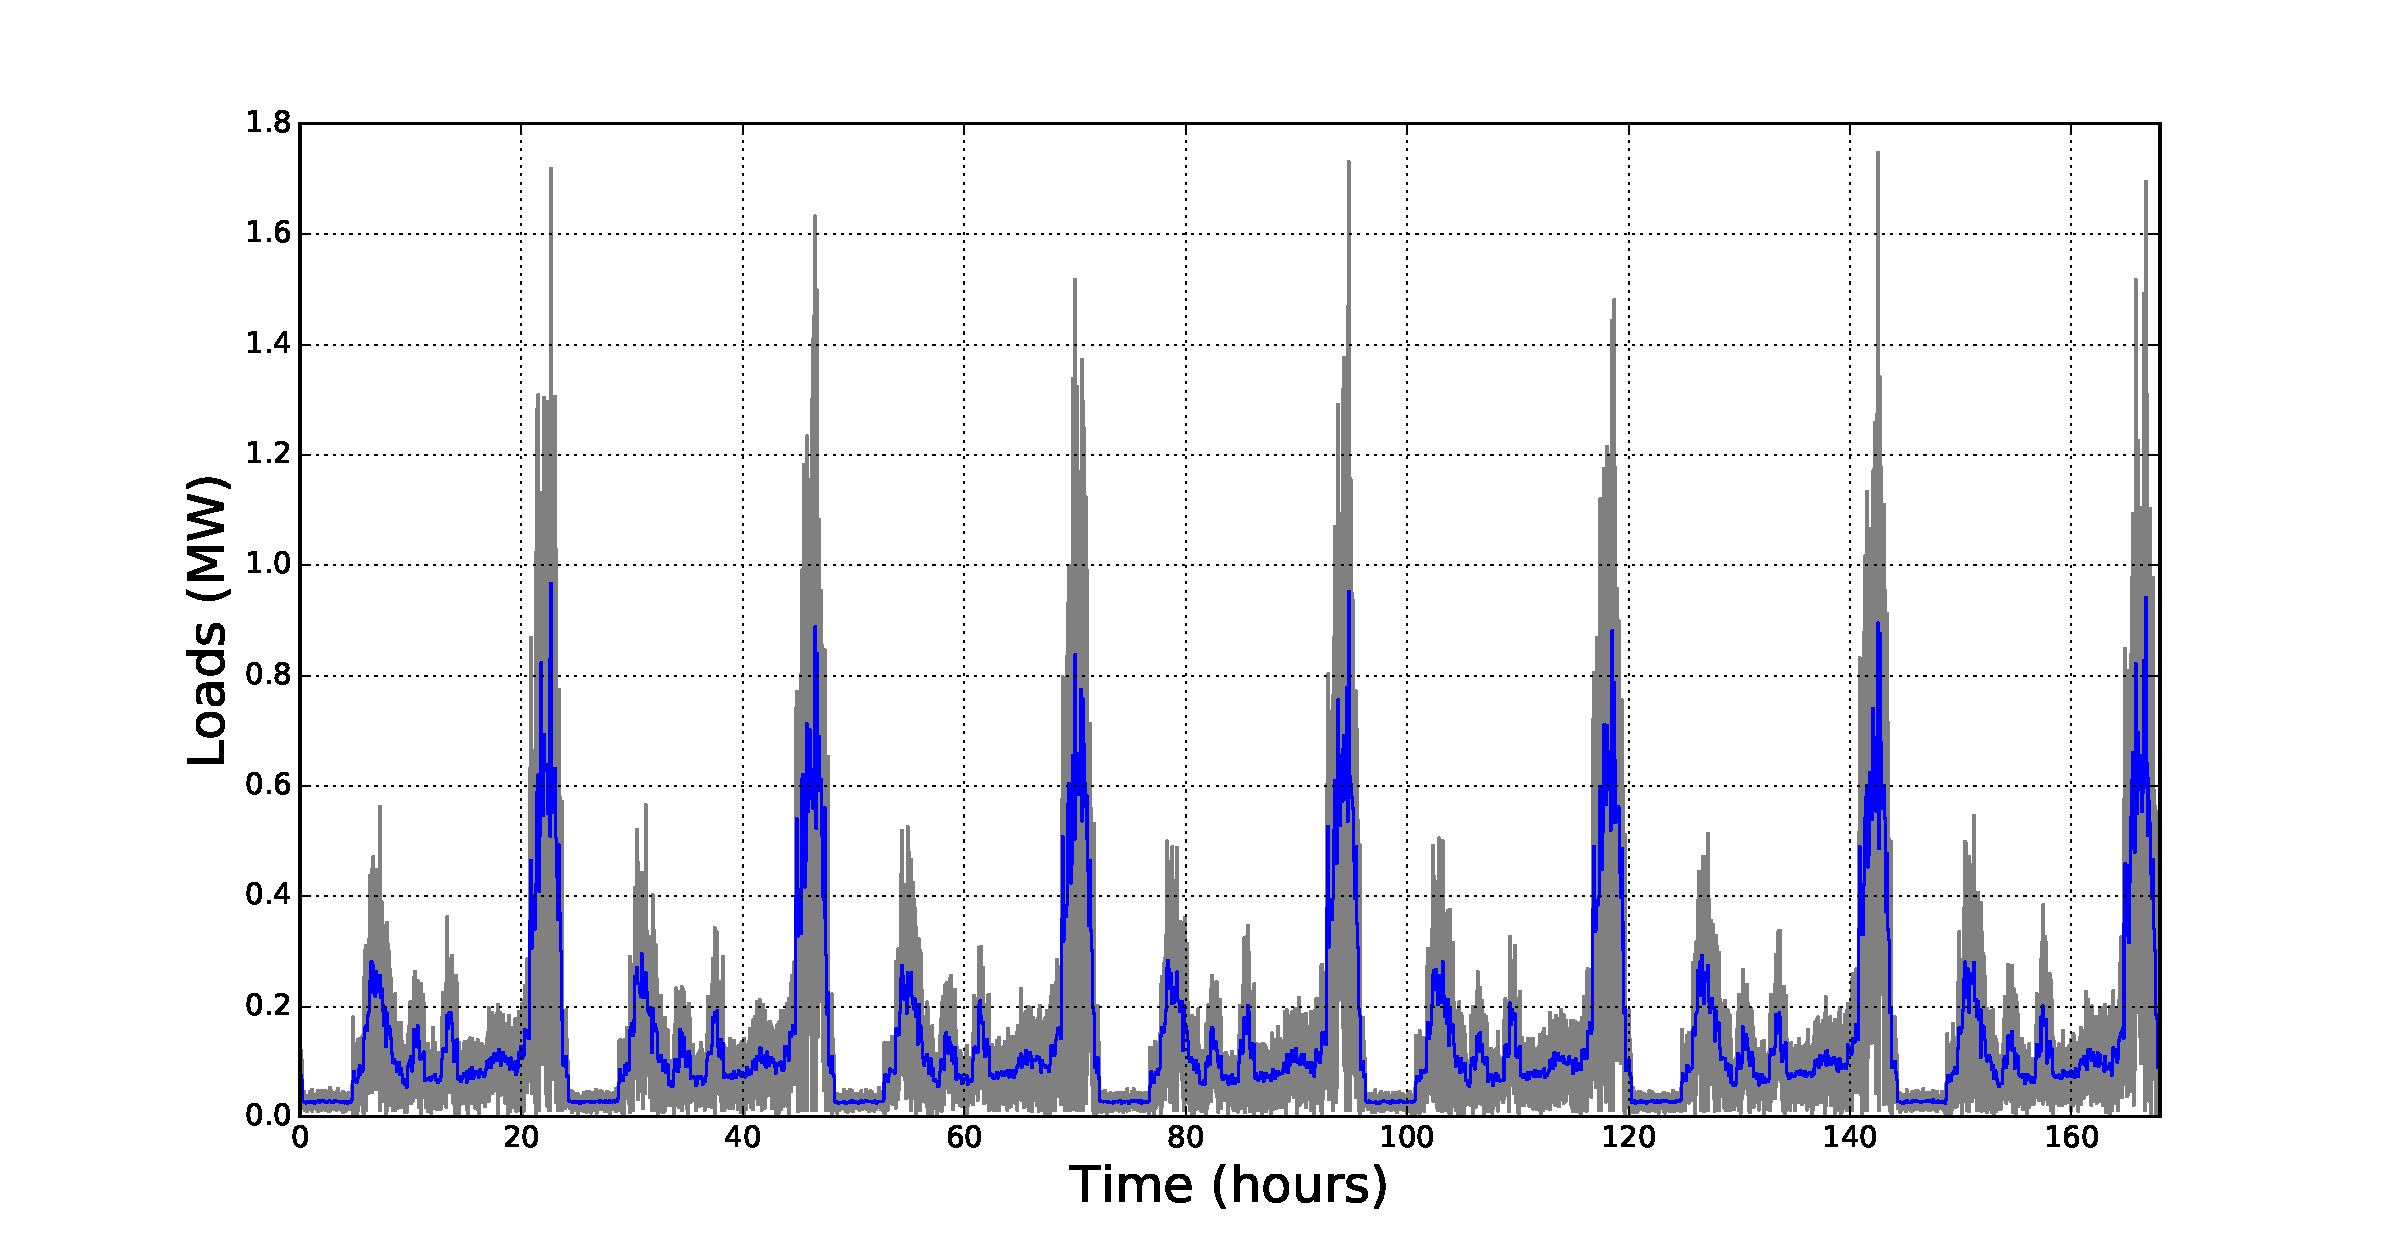
\includegraphics[width=4in]{Figures/Plots/fullproblem_stoch/loads_scenarios.pdf} \caption{Load scenarios for a week}\label{fig:loads_scenarios}\end{center}
\end{figure}

In this work we assume uncertainty only in the load demands and consider the day-ahead market participation to be first stage decision while real time market decision are treated as recourse. The goals of this work include to :
\begin{itemize}
\item Investigate the economic potential of participating in various markets within a stochastic programming setting i.e. compare expected revenue from different markets and explore the benefits of participating in both real time and day-ahead markets
\item Employ different multi-stage stochastic optimization solution methods and compare their performance. The methods compared are:
\begin{itemize}
\item Sample average approximation of extensive form
\item Upper and lower bound estimations using perfect information and two-stage approximation (restriction)
\item Stochastic dual dynamic programming (SDDP)
\item Receding horizon 
\end{itemize}
\end{itemize}

\section{Optimization Model for Building-Battery System}\label{sec:model}
\subsection{Deterministic Setting}\label{subsec:deterministic}
First, we formulate an optimization problem to minimize the cost (or maximize revenue) for the building-battery system operating in the electricity market in a deterministic setting assuming no uncertainty in any of the market and demand quantities. In this formulation, the building-battery system participates in the market at two timescales, hourly and 5-minute intervals. Since the price and load signals are discrete, real-time prices and loads available at 5-minute intervals and day-ahead prices at hourly intervals, we make the zero-order hold assumption, i.e. these time-varying signals are constant within an interval of corresponding duration of their timescale. We also assume that the energy stored in the battery before beginning of market participation is fixed at $E_{0}$. The building-battery system is illustrated with a schematic diagram in Figure \ref{fig:system}.

With these assumptions, we develop the optimization problem formulation for the system is described below.
\subsubsection{Sets used in the model}
\begin{center}
$\mathcal{T_R} := \{1,..,n_{\textrm{rtm}}\}$\\$ \mathcal{T_D} :=  \{1,..,n_{\textrm{dam}}\}$
\end{center}
Here, $\mathcal{T_R}$ is the set of time indices corresponding to each 5-minute subintervals in the real-time market within each hour, so $n_{rtm}=12$. $\mathcal{T_D}$ is the set of time indices corresponding to the hourly intervals of the day-ahead market. $n_d$ can be chosen appropriately for any number of hours we plan to schedule the market participation policy for the building-battery system.
\subsubsection{Time discretization used in the model}
A time instance for a day-ahead market variable in the model is represented by only the index $k$ ($k \in \mathcal{T_D}$) which corresponds to the interval between hours $k-1$ and $k$. On the other hand, a time instance for a real-time variable in the model is represented by index $(i,k)$, where $i \in \mathcal{T_R}$ and $ k \in \mathcal{T_D}$. The indices $i$ and $k$ in a time instance $(i,k)$ for a real-time variable correspond to the end of the respective 5-minute interval. For example, the time instance ($5,7$) corresponds to the end of the interval between $4^{\text{th}}$ and $5^{\text{th}}$ 5-minute interval within the $7^\textrm{th}$ hour. 

So, if a variable or time-varying parameter is indexed by only one index $k$ it implies that it varies at hourly intervals and belongs to the day-ahead market, whereas a variable or time-varying parameter indexed by $(i,k)$ is a real-time variable. 

The time discretization and zero-order hold have been illustrated for the battery power in real-time and day-ahead markets in Figure \ref{fig:discretization}.
\begin{figure}[h!]
\begin{center}
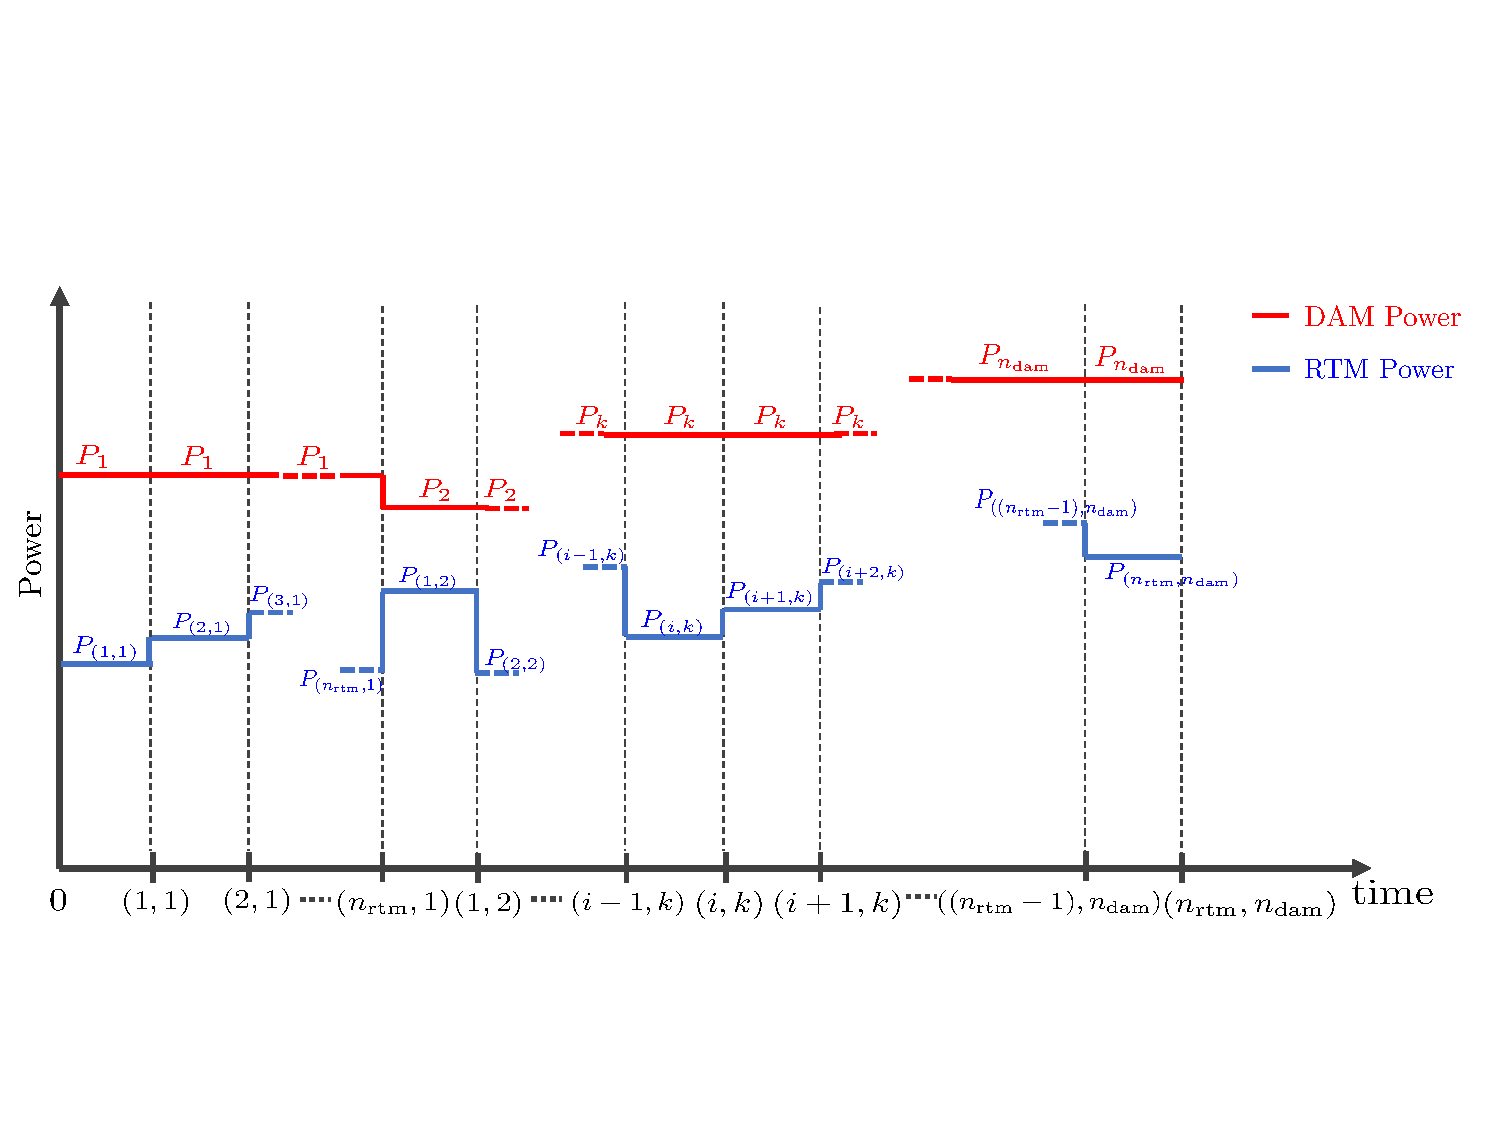
\includegraphics[scale=0.7]{Figures/discretization1.pdf} \caption{Time Discretization and Zero-Order Hold for Variables}\label{fig:discretization}\end{center}
\end{figure}
\FloatBarrier
\subsubsection{Parameters in the model:}
\begin{itemize}
\item\textbf{Market parameters:}
\begin{itemize}
\item[\textbullet] $\pi_{k}, \forall k \in \mathcal{T_D}$: Electricity price in day-ahead market in the interval between hour $k-1$ to $k$
\item[\textbullet] $\pi_{i,k}, \forall i \in \mathcal{T_R}, k \in \mathcal{T_D}$: Electricity price in real-time market in the 5-minute interval between $(i-1,k)$ and $(i,k)$ within $k^\text{th}$ hour
\item[\textbullet] $\Delta t$: Time interval (in unit of hours) in the real-time market (which is 5 minutes)
\end{itemize}
\item\textbf{Battery parameters:}
\begin{itemize}
\item[\textbullet] $E_{max} = 0.5$ MWh: Energy storage capacity of the battery
\item[\textbullet] $P_{max} = 0.5$ MW: Maximum discharging or charging rate of the battery
\item[\textbullet] $E_{0} = E_{max}$: Energy stored in the battery before beginning of market participation
\end{itemize}
\item\textbf{Building loads:}
\begin{itemize}
\item[\textbullet] $L_{i,k}, \forall i \in \mathcal{T_R}, k \in \mathcal{T_D}$: Building loads in the 5-minute interval between $(i-1,k)$ and $(i,k)$ within $k^\text{th}$ hour
\end{itemize}
\end{itemize}
\subsubsection{Variables in the model:}
\begin{itemize}
\item \textbf{Decision variables:}
\begin{itemize}
\item[\textbullet] $P_{k}, \forall k \in \mathcal{T_D}$: Power committed by battery in day-ahead market in the interval between hour $k-1$ to $k$
\item[\textbullet] $P_{i,k}, \forall i \in \mathcal{T_R}, k \in \mathcal{T_D}$: Power committed by battery in real-time market in the 5-minute interval between $(i-1,k)$ and $(i,k)$ within $k^\text{th}$ hour
\item[\textbullet] $L^{sup}_{i,k}, \forall i \in \mathcal{T_R}, k \in \mathcal{T_D}$: Power supplied by battery to the building in the 5-minute interval between $(i-1,k)$ and $(i,k)$ within $k^\text{th}$ hour 
\end{itemize}
\item \textbf{State variables:}
\begin{itemize}
\item[\textbullet] $E_{i,k}, \forall i \in \mathcal{T_R}, k \in \mathcal{T_D}$: Energy stored in the battery at time $(i,k)$ (at the end of $i^{th}$ 5-minute interval within $k^\text{th}$ hour) 
\end{itemize}
\end{itemize}
\begin{figure}[h!]
\begin{center}
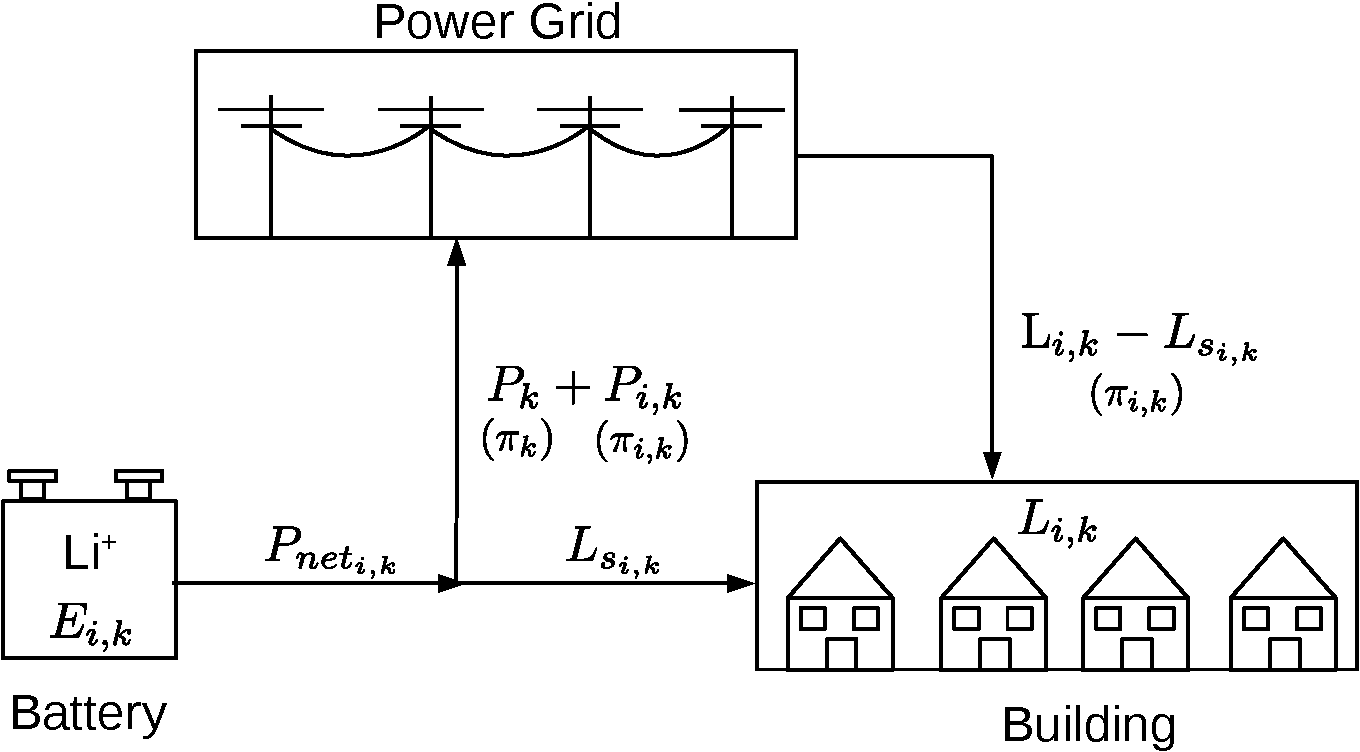
\includegraphics[scale=0.6]{Figures/system_blocks-crop.pdf} \caption{Illustration of Battery-Building System Interconnected with Power Grid}\label{fig:system}\end{center}
\end{figure}
\FloatBarrier
\subsubsection{Constraints and objective function}\label{subsec:const_obj}
\begin{itemize}
\item Net discharge (power) from the battery at any time has to be less than the maximum discharge capacity of the battery, $P_{max}$.
\begin{align}\label{eq:Pnet}
&P_{{net}_{i,k}} = P_{k} + P_{i,k} + L^{sup}_{i,k}, \quad \forall i \in \mathcal{T_R}, k \in \mathcal{T_D}
\end{align}
\item Balance on the energy stored in the battery at each time
\begin{align}\label{eq:ebalance}
E_{i,k} =& E_{i-1,k}- P_{{net}_{i,k}}\Delta t_r, \quad \forall i \in \mathcal{T_R}, k \in \mathcal{T_D}
\end{align}
In Equation \eqref{eq:ebalance}, $E_{0,k} = E_{0}$ for $k \in \lbrace1\rbrace$ and $E_{0,k} = E_{n_{rtm},k-1}$ for $k \in \mathcal{T_R}\setminus{\lbrace1\rbrace}$. 
\item Bounds on variables:
\begin{subequations}\label{eq:bounds}
\begin{align}
0 & \leq E_{i,j,k} \leq E_{max}, \forall i \in \mathcal{T_R}, k \in \mathcal{T_D}\\
-P_{max} & \leq P_{i,k} \leq P_{max}, \forall i \in \mathcal{T_R}, k \in \mathcal{T_D}\\
-P_{max} & \leq P_{k}\phantom{i,} \leq P_{max}, \forall k \in \mathcal{T_D}\\
-P_{max} & \leq P_{{net}_{i,k}} \leq P_{max}, \forall i \in \mathcal{T_R}, k \in \mathcal{T_D}\\
0 & \leq L^{sup}_{i,k} \leq L_{i,k}, \forall i \in \mathcal{T_R}, k \in \mathcal{T_D}
\end{align}
\end{subequations}
\item Objective Function:
\begin{align}\label{objective}
\min \quad -\sum\limits_{i \in \mathcal{T_R}}\sum\limits_{k \in \mathcal{T_R}} \pi_{i,k}P_{i,k}\Delta t_r - \sum\limits_{k \in \mathcal{T_D}}\pi_{k}P_{k}\Delta t_r n_{rtm} + \sum\limits_{i \in \mathcal{T_R}}\sum\limits_{k \in \mathcal{T_R}} \pi_{i,k}(L_{i,k}-L^{sup}_{i,k})\Delta t_r
\end{align}
\end{itemize}

\subsection{Optimization Model Under Uncertainty} \label{subsec:opt_unc}
Now, we consider uncertainty in the building loads and extend the optimization formulation in deterministic setting (Section \ref{subsec:deterministic}) to formulate an extensive form of stochastic optimization problem to minimize the expected cost (or maximize expected revenue) for the building-battery system. In the formulation for the optimization problem under uncertainty, we consider all the the market participating conditions to be the same as in the deterministic setting except for the uncertainty in the loads. We use the same sets of time indices, time-discretization approach and variable/parameter notations as developed in Section \ref{subsec:deterministic} with the exception that uncertainty has to be added to all real-time variables because of the uncertain loads. We represent this uncertainty with a sample space $\Xi$ and an outcome from this space is denoted by $\xi$. As described in Section \ref{sec:setting}, we consider that when a scenario $\xi \in \Xi$ realizes at an hour $k$ the loads at all real-time subintervals between hour $k-1$ and $k$ become known and the scenario-tree grows at every hour. So, the uncertain load at every time is denoted as $L_{i,k}(\xi)$. Similarly, we denote the resulting uncertainty in all real-time variables, namely the energy transacted by the battery with real-time market ($P_{i,k}(\xi)$), the energy supplied by the battery to the building ($L^{sup}_{i,k}(\xi)$) and the energy stored in the battery at every time ($E_{i,k}(\xi)$). The day-ahead energy participation by the battery is a first-stage decision which needs to be made before the realization of uncertainty. Furthermore, for the extensive form of the stochastic programming model, we assume that the uncertainty can be represented by a set of $N$ possible scenarios $\mathcal{S}$ and all possible realizations of uncertainty lies in this set. So, $s \in \mathcal{S}$ represents a possible scenario of the realization of uncertainty. Also, we make the assumption that the scenarios are equiprobable. We use these assumptions to build the extensive form of the stochastic program to minimize the expected cost (maximize expected revenue) for the system and is described below.

\subsubsection{Variables in the extensive form model}\label{subsubsec:var_ext}
\begin{itemize}
\item \textbf{Decision variables:}
\begin{itemize}
\item[\textbullet] $P_{k,s}, \forall k \in \mathcal{T_D}, \forall s \in \mathcal{S}$: Power committed by battery in day-ahead market in the interval between hour $k-1$ to $k$ in scenario $s$
\item[\textbullet] $P_{i,k,s}, \forall i \in \mathcal{T_R}, k \in \mathcal{T_D}, \forall s \in \mathcal{S}$: Power committed by battery in real-time market in the 5-minute interval between $(i-1,k)$ and $(i,k)$ within $k^\text{th}$ hour in scenario $s$
\item[\textbullet] $L^{sup}_{i,k,s}, \forall i \in \mathcal{T_R}, k \in \mathcal{T_D}, \forall s \in \mathcal{S}$: Power supplied by battery to the building in the 5-minute interval between $(i-1,k)$ and $(i,k)$ within $k^\text{th}$ hour in scenario $s$
\end{itemize}
\item \textbf{State variables:}
\begin{itemize}
\item[\textbullet] $E_{i,k,s}, \forall i \in \mathcal{T_R}, k \in \mathcal{T_D}, \forall s \in \mathcal{S}$: Energy stored in the battery at time $(i,k)$ (at the end of $i^{th}$ 5-minute interval within $k^\text{th}$ hour)  in scenario $s$
\end{itemize}
\end{itemize}

\subsubsection{Constraints and objective function}\label{subsubsec:const_obj_ext}
\begin{itemize}
\item Net discharge (power) from the battery at any time has to be less than the maximum discharge capacity of the battery, $P_{max}$.
\begin{align}\label{eq:Pnet_unc}
&P_{{net}_{i,k,s}} = P_{k,s} + P_{i,k,s} + L^{sup}_{i,k,s}, \quad \forall i \in \mathcal{T_R}, k \in \mathcal{T_D}, s \in \mathcal{S}
\end{align}
\item Balance on the energy stored in the battery at each time
\begin{align}\label{eq:ebalance_unc}
E_{i,k,s} =& E_{i-1,k,s}- P_{{net}_{i,k,s}}\Delta t_r, \quad \forall i \in \mathcal{T_R}, k \in \mathcal{T_D}, s \in \mathcal{S}
\end{align}
In equation \eqref{eq:ebalance_unc}, $E_{0,k,s} = E_{0}$ for $k \in \lbrace1\rbrace$ and $E_{0,k,s} = E_{n_{rtm},k-1,s}$ for $k \in \mathcal{T_R}\setminus{\lbrace1\rbrace}$. 
\item Bounds on variables:
\begin{subequations}\label{eq:bounds_unc}
\begin{align}
0 & \leq E_{i,j,k,s} \leq E_{max}, \forall i \in \mathcal{T_R}, k \in \mathcal{T_D}\\
-P_{max} & \leq P_{i,k,s} \leq P_{max}, \forall i \in \mathcal{T_R}, k \in \mathcal{T_D}, s \in \mathcal{S}\\
-P_{max} & \leq P_{k,s}\phantom{i,} \leq P_{max}, \forall k \in \mathcal{T_D}, s \in \mathcal{S}\\
-P_{max} & \leq P_{{net}_{i,k,s}} \leq P_{max}, \forall i \in \mathcal{T_R}, k \in \mathcal{T_D}, s \in \mathcal{S}\\
0 & \leq L^{sup}_{i,k,s} \leq L_{i,k,s}, \forall i \in \mathcal{T_R}, k \in \mathcal{T_D}, s \in \mathcal{S}
\end{align}
\end{subequations}
\item Nonanticipativity constraints for first-stage decisions ($P_{k,s}$):
\begin{align}\label{eq:nonant_unc}
P_{k,s} =& \frac{1}{N} \sum\limits_{s \in \mathcal{S}} P_{k,s}, \quad \forall k \in \mathcal{T_D}, s \in \mathcal{S}
\end{align}
\item Objective Function:
\begin{align}\label{objective_unc}
\min \quad \frac{1}{N} \sum\limits_{s \in \mathcal{S}} \left[-\sum\limits_{i \in \mathcal{T_R}}\sum\limits_{k \in \mathcal{T_R}} \pi_{i,k}P_{i,k,s}\Delta t_r - \sum\limits_{k \in \mathcal{T_D}}\pi_{k}P_{k,s}\Delta t_r n_{rtm} + \sum\limits_{i \in \mathcal{T_R}}\sum\limits_{k \in \mathcal{T_R}} \pi_{i,k}(L_{i,k,s}-L^{sup}_{i,k,s})\Delta t_r \right]
\end{align}
\end{itemize}

\section{Computational Experiments}\label{sec:exp}

\subsection{Economic Potential of Different Timescales of Electricity Markets}
In this case study, we sample 50 scenario paths (out of the $50^{168}$ possibilities) for a week's time period. We then construct a full model for for this week and use real price signals from 01/01/2015 to 01/07/2015 in California ISO \footnote{http://oasis.caiso.com/mrioasis/logon.do}. For every 1 hour interval in the model, we sample a scenario, and use the load data corresponding to that scenario for the 12 intervals (5 minutes each) in that hour. This helps to reduce the size of scenario tree (from $50^{168 \times 12}$ to $50^{168}$). We solve this model (with 50 sampled paths) 100 times to get a confidence interval on the expected revenue. We then compare this expected revenue (obtained by participating in both real time and day-ahead market) to the cases when the battery participates only in either real time or day-ahead market alone.
\begin{table}[!ht]\centering
\caption{Revenue Breakup from Participation in Different Markets}
\begin{tabular}{|C{3cm}|C{2.5cm}|C{3.5cm}|C{3cm}|C{2.5cm}|} 
\hline 
Market Participated  & Total Revenue (\$) & Unmet Load Cost (\$) & DAM Revenue  (\$) & RTM Revenue (\$) \\
\hline 
DAM + RTM & 711.08 & -8.75 & 793.12 & -90.79 \\ 
\hline 
DAM & -921.73 & 77.00 & -844.73 & N/A \\ 
\hline 
RTM & -31.32 & -9.10 & N/A & -40.42 \\ 
\hline 
None & -10,293.23 & 10,293.23 & N/A & N/A \\ 
\hline 
\end{tabular} \label{tab:rev_comp} 
\end{table}
Highest revenue is earned when the battery participates in both the real time and day-ahead markets (Table \ref{tab:rev_comp}). Whereas, if it participates in just day-ahead or real time market alone, the revenue is much less or even negative (results in loss). Consider the case when it participates in only day ahead market. It is evident from Figure \ref{fig:Pdam_onlydam} and \ref{fig:cumulative_rev_onlydam} that the battery needs to charge itself (buy energy from the grid) in order to meet the building load demands. The price of energy is on average higher in day-ahead market than that in real time markets. Thus with no participation in real time market in does not have the flexibility to buy energy from the real-time market at lower prices and sell to day-ahead market (at a higher price) to make profits. The building loads need to be met in real-time (at every 5-minute interval) while the battery has the opportunity to buy or sell energy from the grid only at every hour. Thus the battery is forced to store enough energy to meet the building requirement for an hour by buying energy in hourly intervals from the day-ahead market. Whenever it has slightly excess energy available it tries to sell that energy to the day-ahead market to minimize the overall cost. 

On the other hand, when it participates in both day-ahead and real-time markets, it has the flexibility to buy from the real-time market and sell to the day-ahead market while saving sufficient energy to meet the building requirement in real-time. This is possible because the real-time electricity prices are slightly lower than the day-ahead market prices on average. The real-time prices also fall below the day-ahead market prices very often (Figures \ref{fig:Pdam_fp_st} and \ref{fig:Prtm_fp_st}) and because of its fast dynamics, the battery can capture these moments by buying from real-time market and selling in day-ahead market to make profit. 
conclusion: market participation in both time scales is important for maximizing the economic potential. The typical problem size in a stochastic setting (considering only 50 samples of load scenarios) for 1 week planning is of the order :
variable: 520900
linear constraints: 722500
time: 37.5 sec (35 - 40 by gurobi)
if there were more number of scenarios, the problem size would grow exponentially. thus for this simultaneous type of problem, we use advanced stochastic techniques to solve these kind of problem. and compare their performance wrt time and expected revenue.
\begin{figure}[h!]
\begin{center}
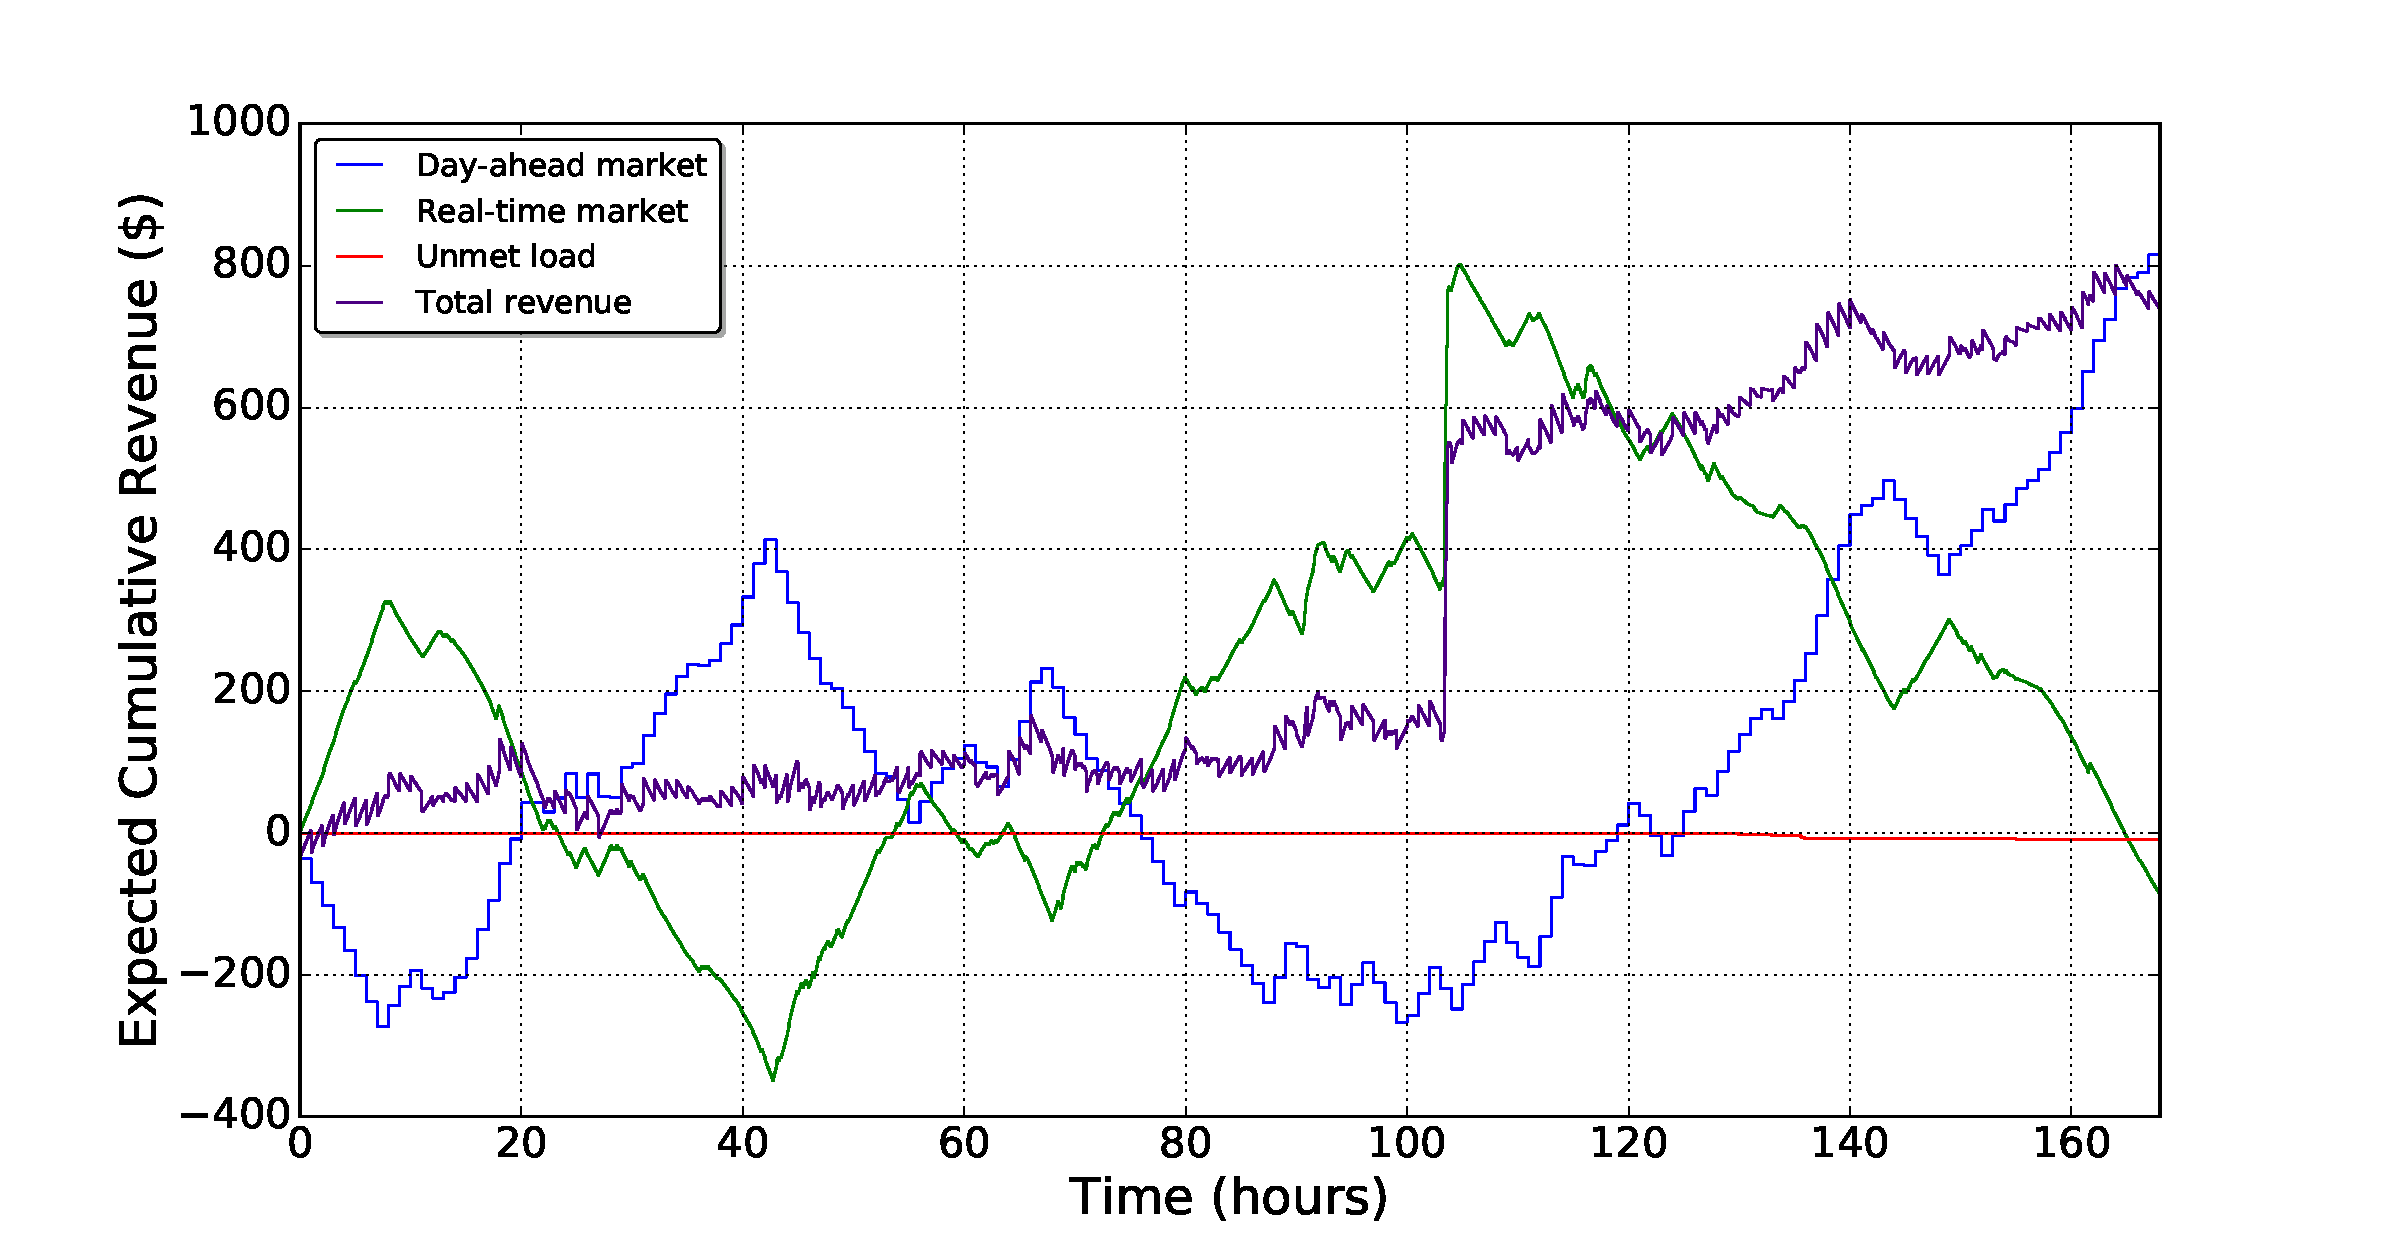
\includegraphics[scale=0.4]{Figures/Plots/fullproblem_stoch/cumulative_rev_fp_st.pdf} \caption{Trajectory of cumulative revenues when battery participates in both day-ahead and real-time markets}\label{fig:cumulative_rev_fp_st}\end{center}
\end{figure}

\begin{figure}[h!]
\begin{subfigure}{\textwidth}
\centering
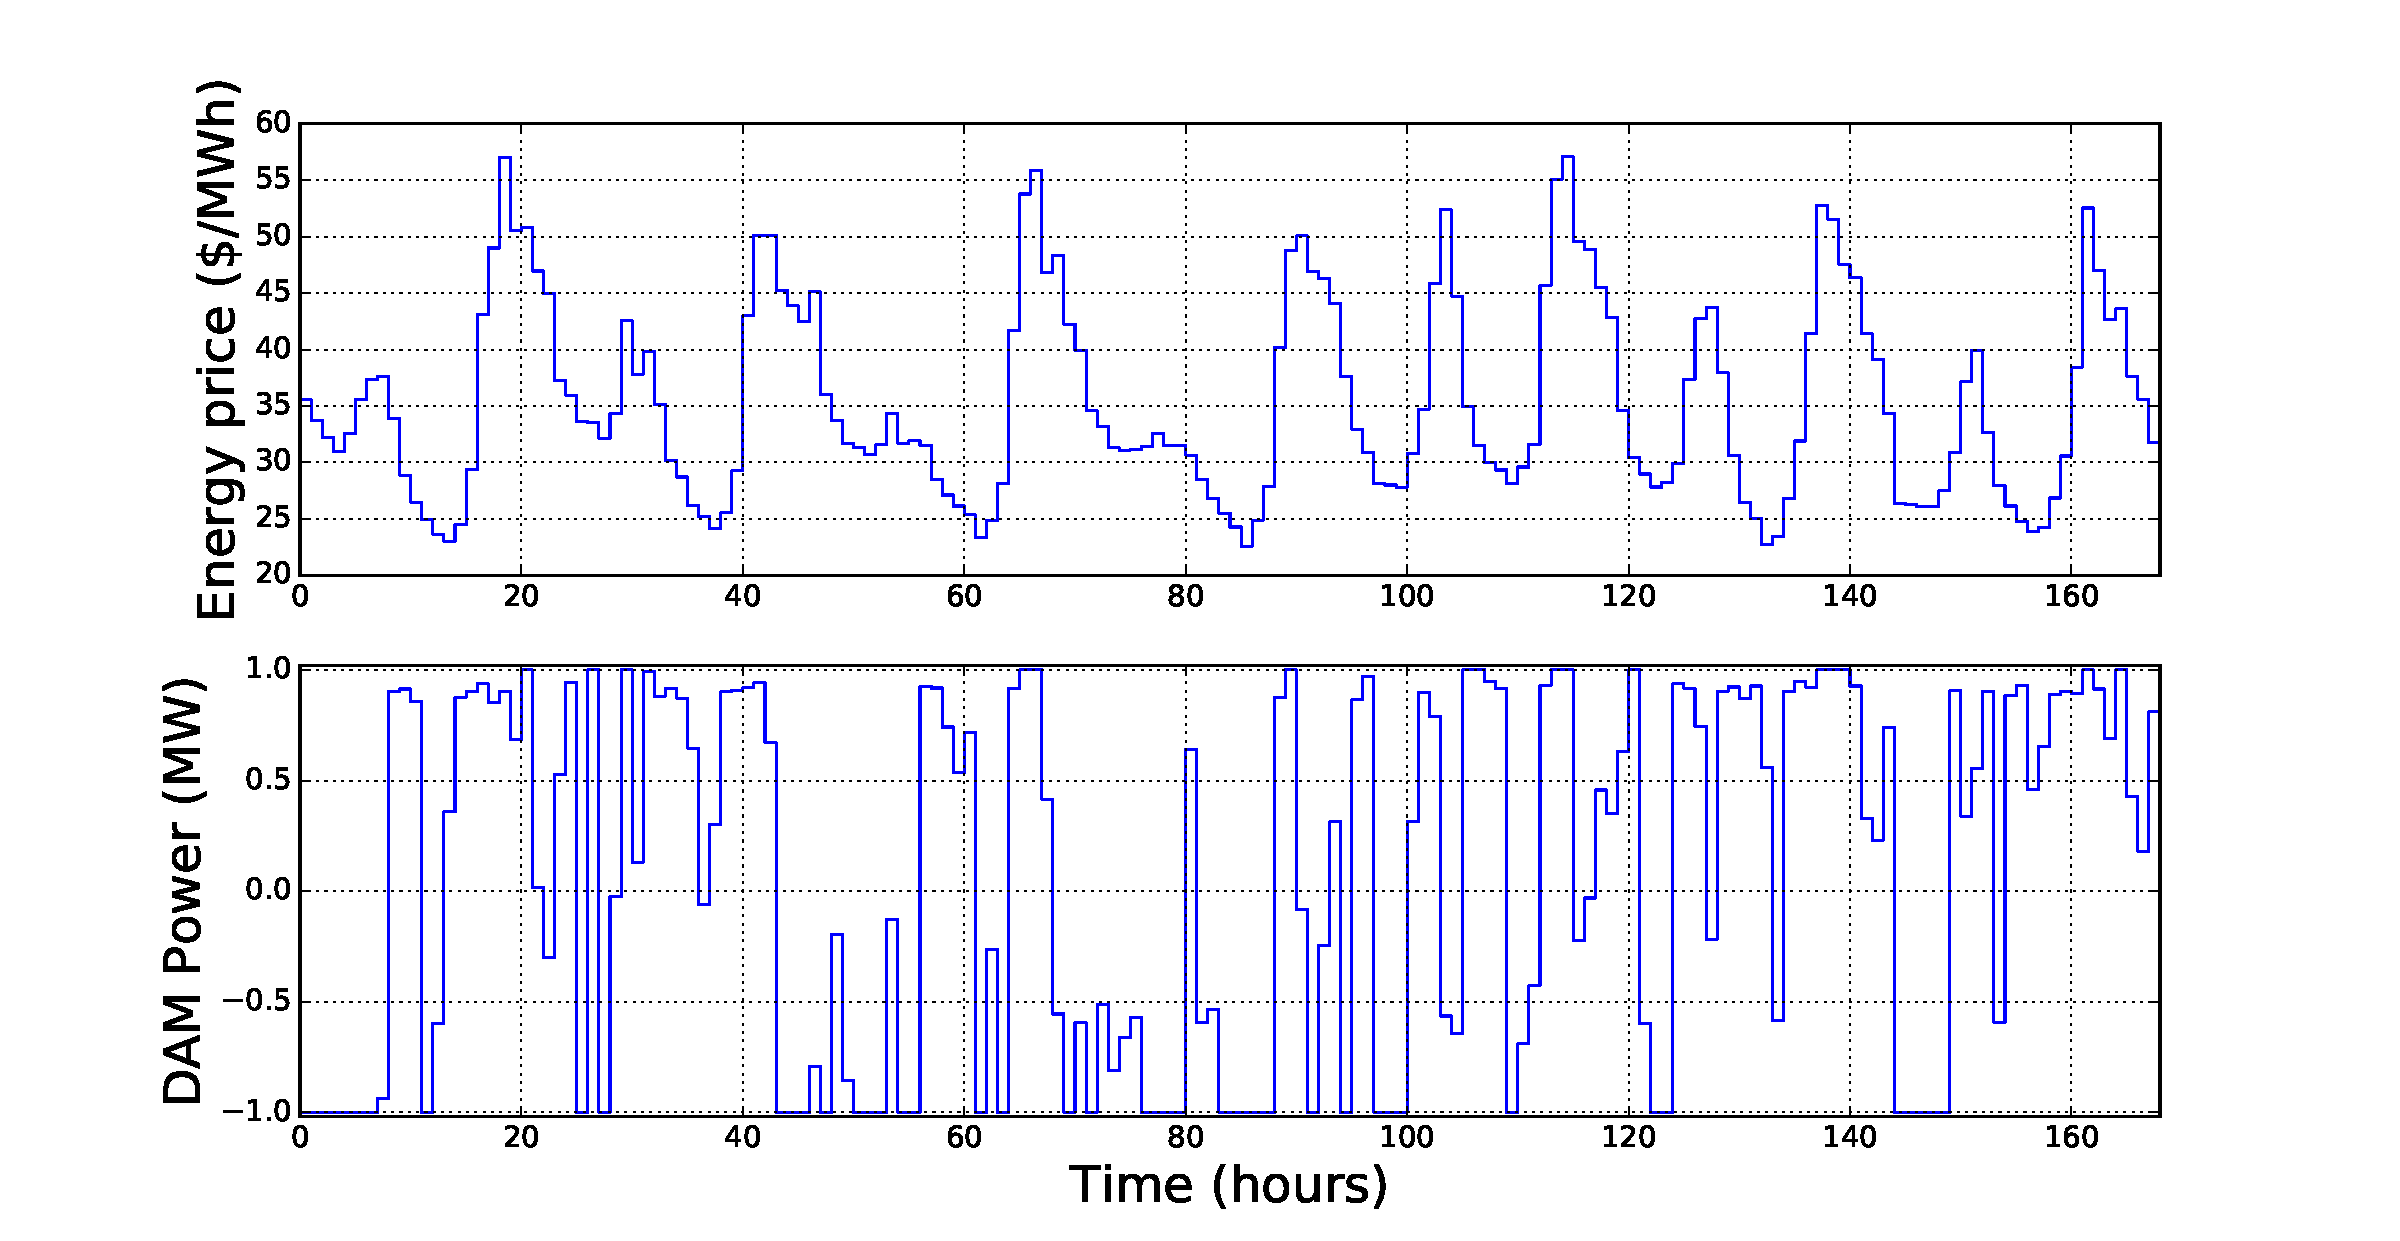
\includegraphics[width=\linewidth]{Figures/Plots/fullproblem_stoch/Pdam_fp_st.pdf} \caption{Day-ahead market}\label{fig:Pdam_fp_st}
\end{subfigure}
\begin{subfigure}{\textwidth}
\centering
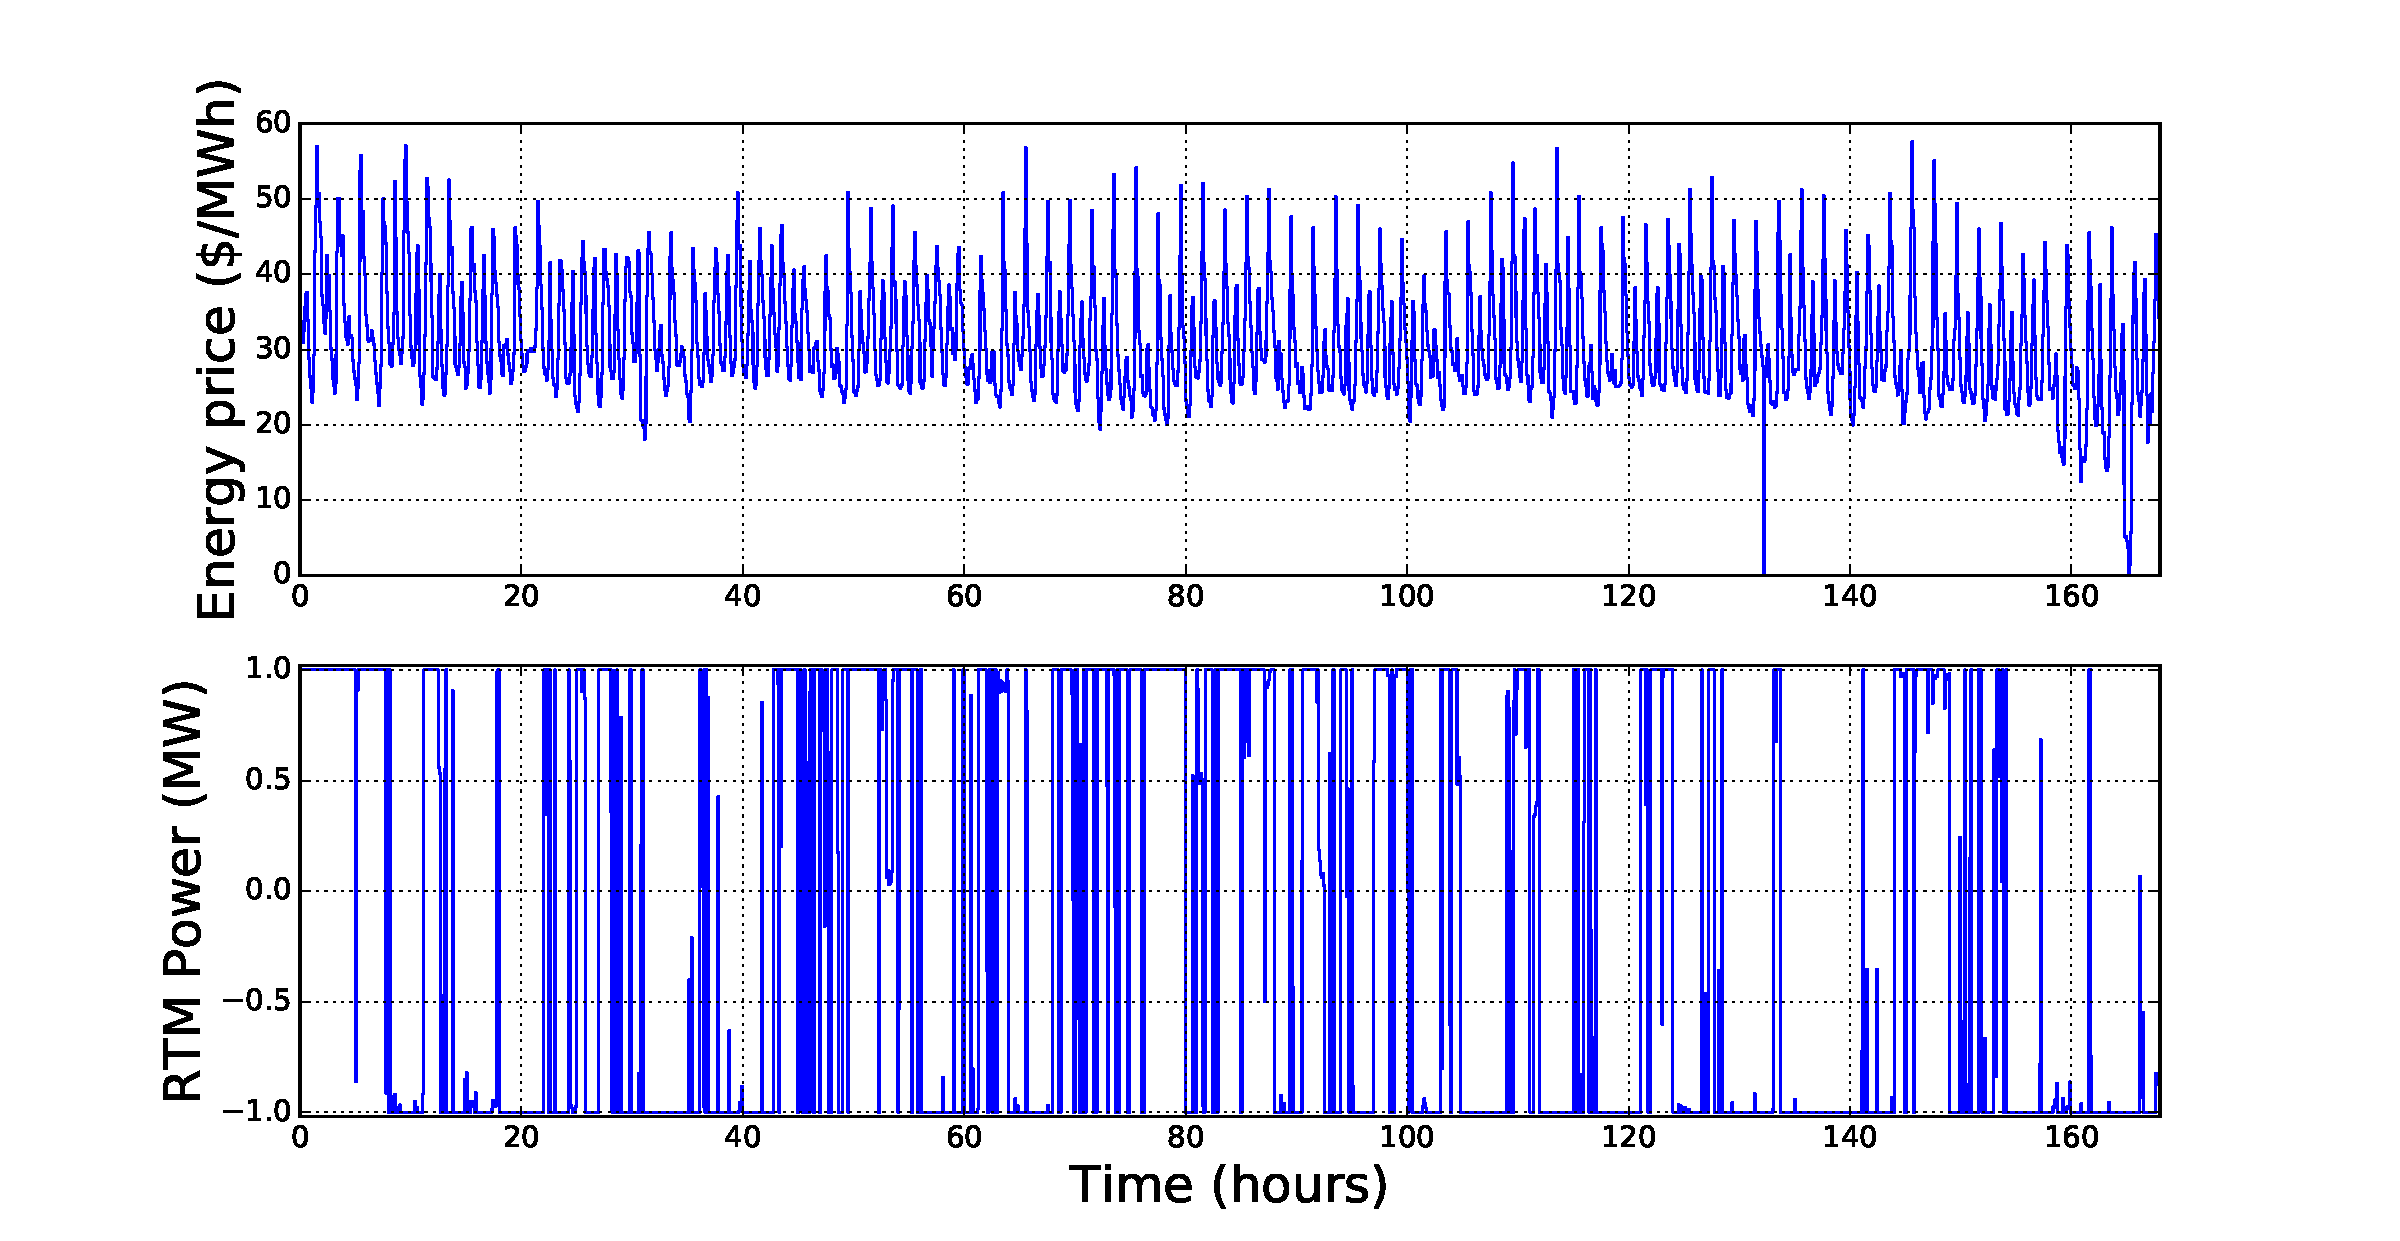
\includegraphics[width=\linewidth]{Figures/Plots/fullproblem_stoch/Prtm_fp_st.pdf} \caption{Real-time market}\label{fig:Prtm_fp_st}
\end{subfigure}
\caption{Energy participation policy when battery participates in both day-ahead and real-time markets}
\end{figure}
\FloatBarrier
\begin{figure}[h!]
\begin{center}
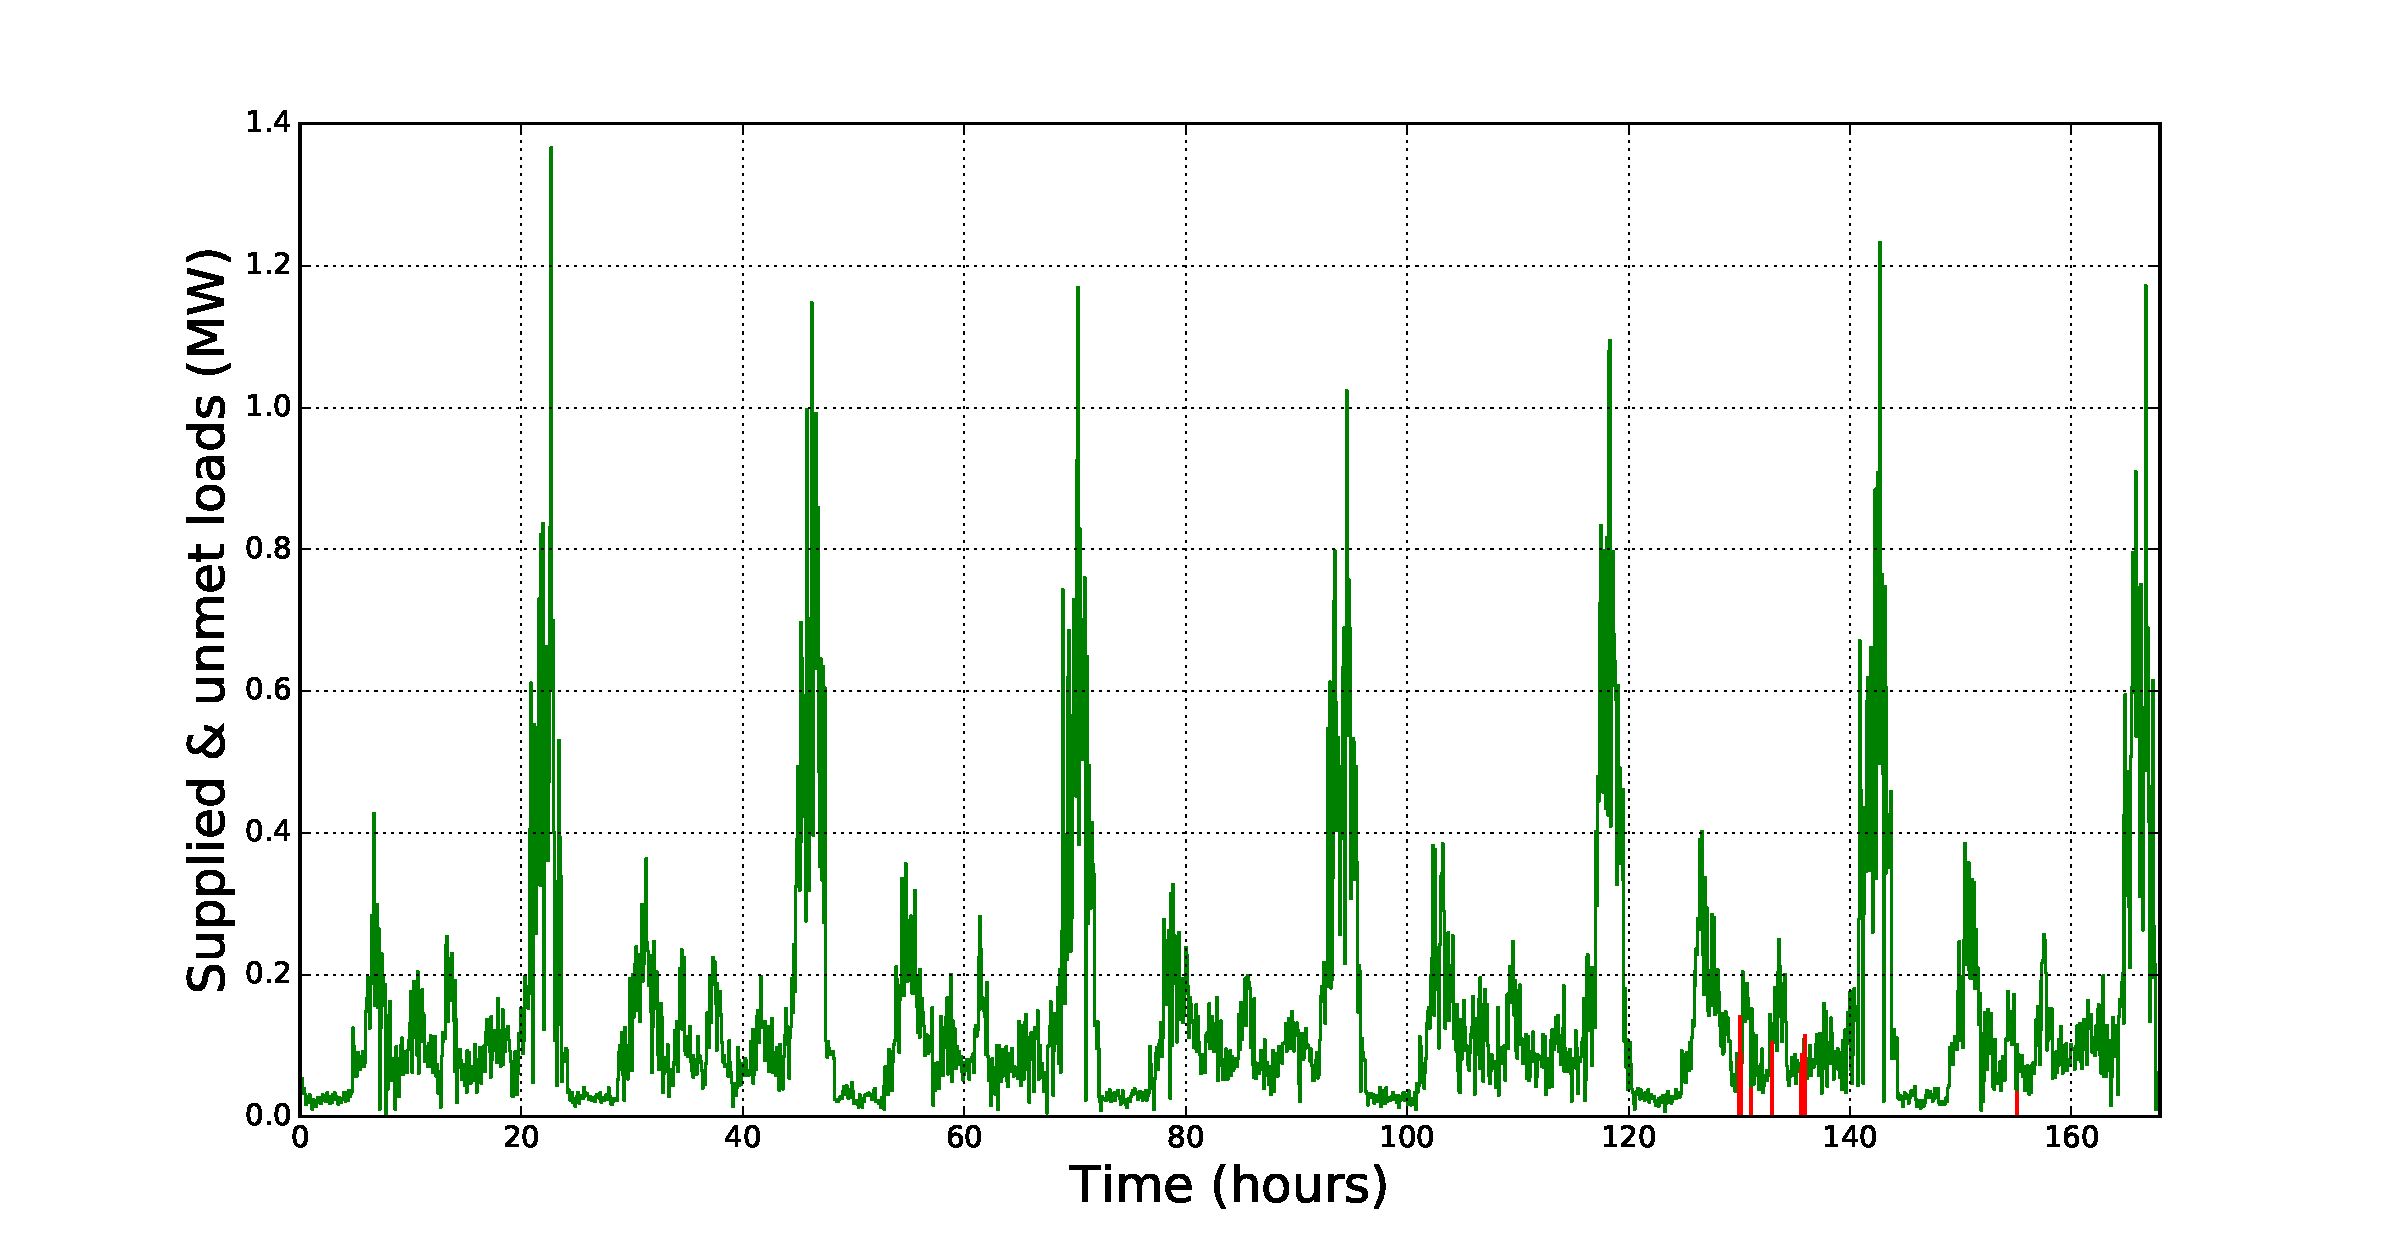
\includegraphics[scale = 0.4]{Figures/Plots/fullproblem_stoch/supp_unmet_fp_st.pdf} \caption{Power supplied to building and unmet load when battery participates in both day-ahead and real-time markets}\label{fig:supp_unmet_fp_st}
\end{center}
\end{figure}

\begin{figure}[h!]
\begin{subfigure}{\textwidth}
\centering
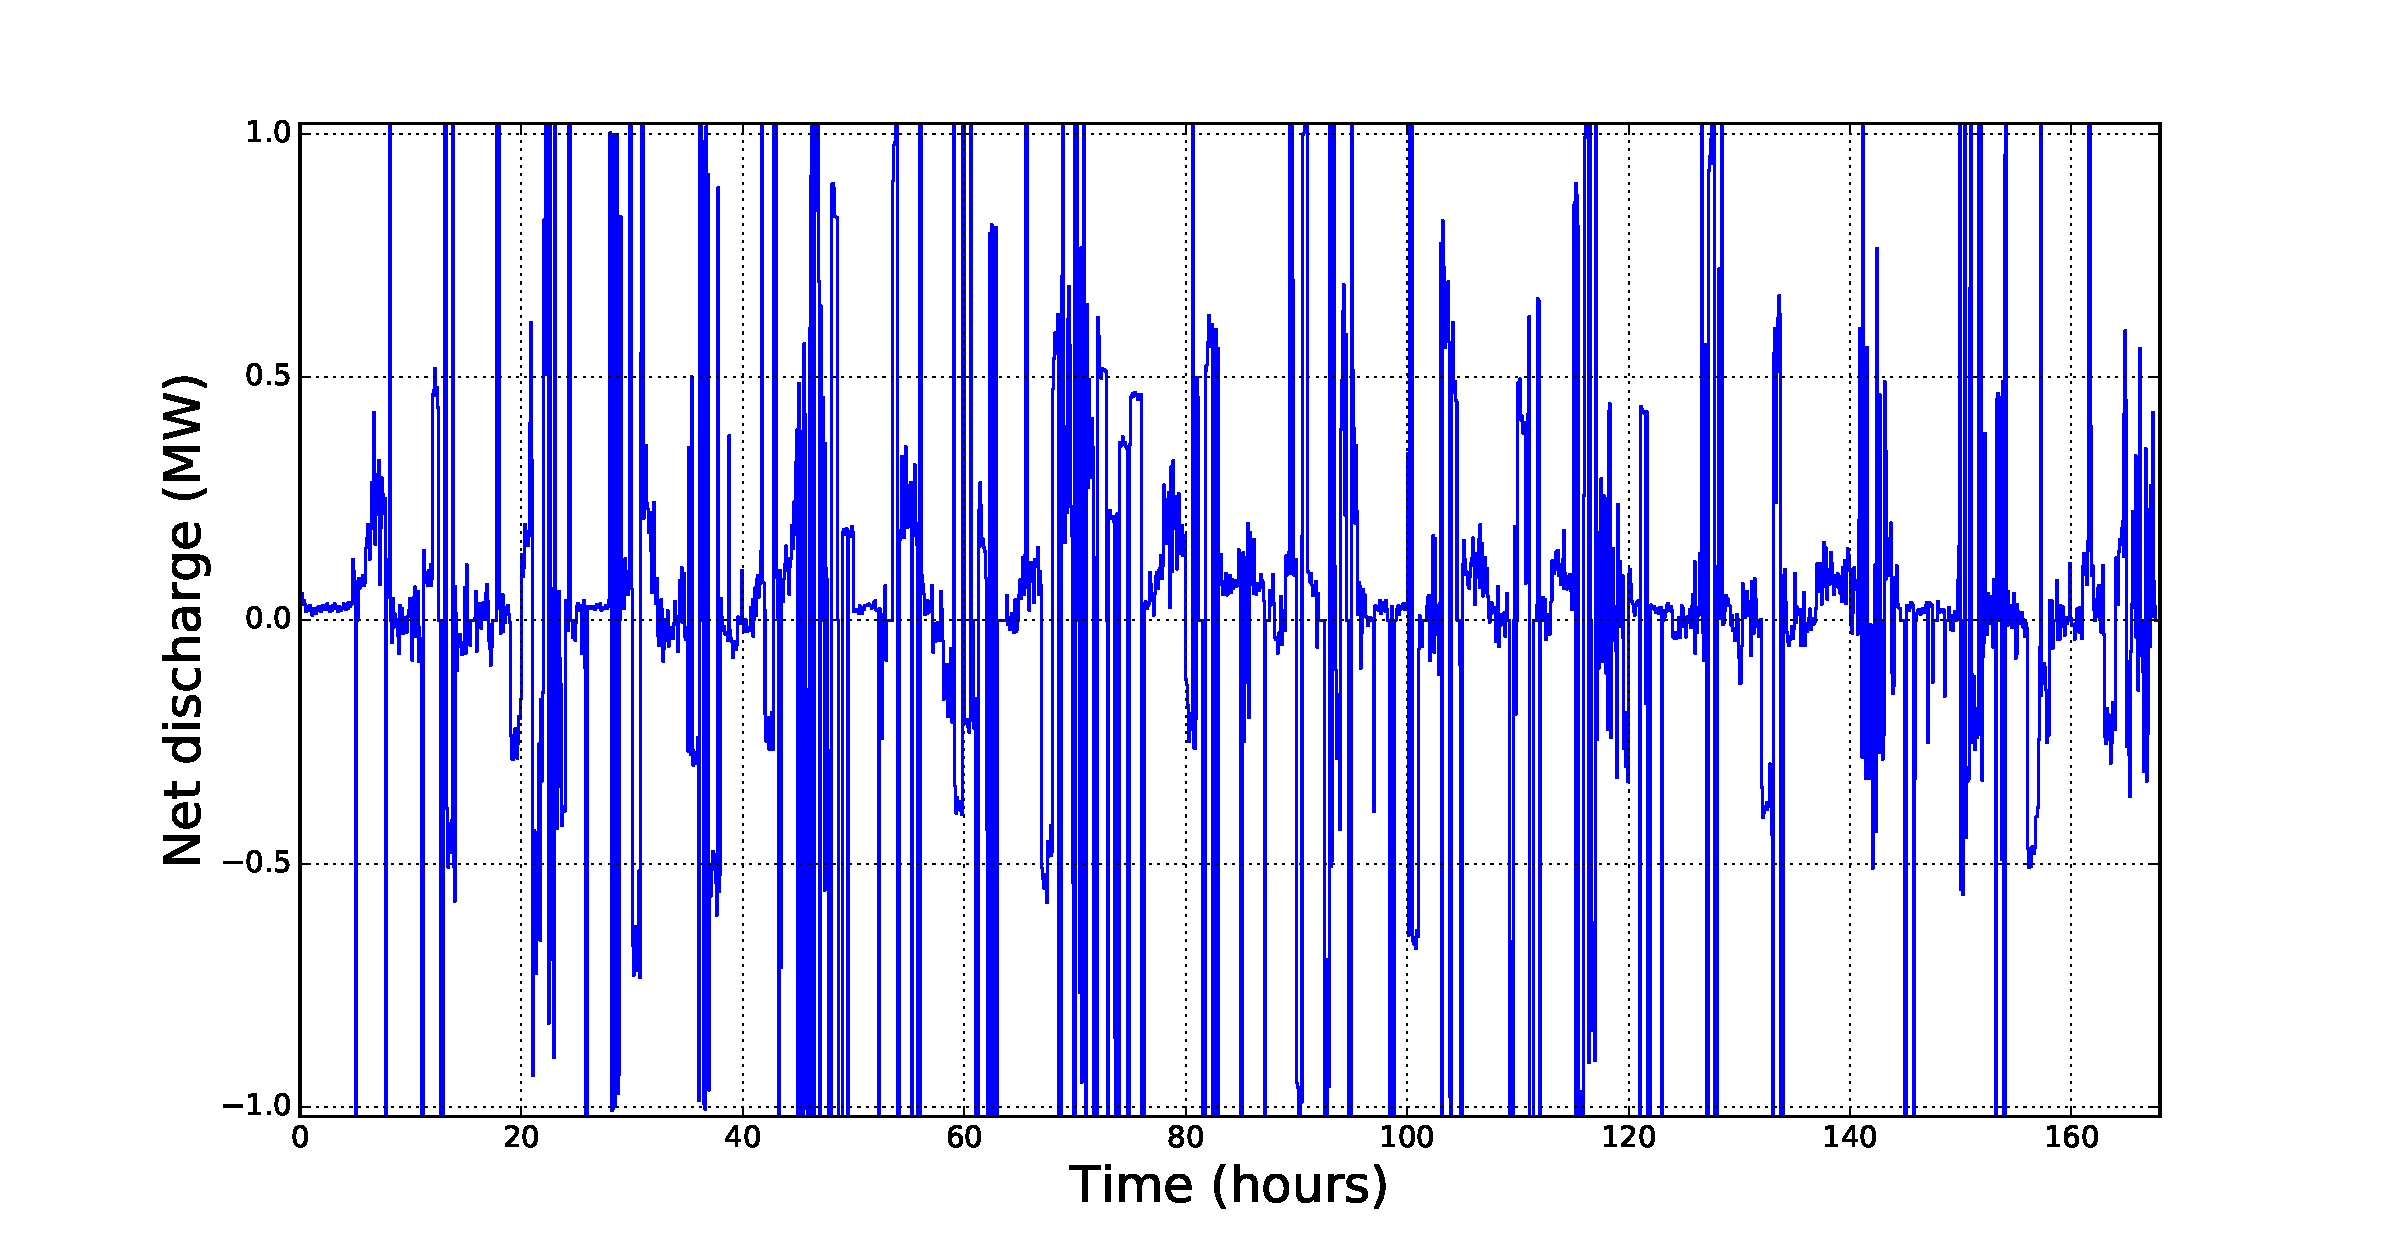
\includegraphics[width=\linewidth]{Figures/Plots/fullproblem_stoch/netpower_fp_st.pdf} \caption{Net battery discharge}\label{fig:netpower_fp_st}
\end{subfigure}
\begin{subfigure}{\textwidth}
\centering
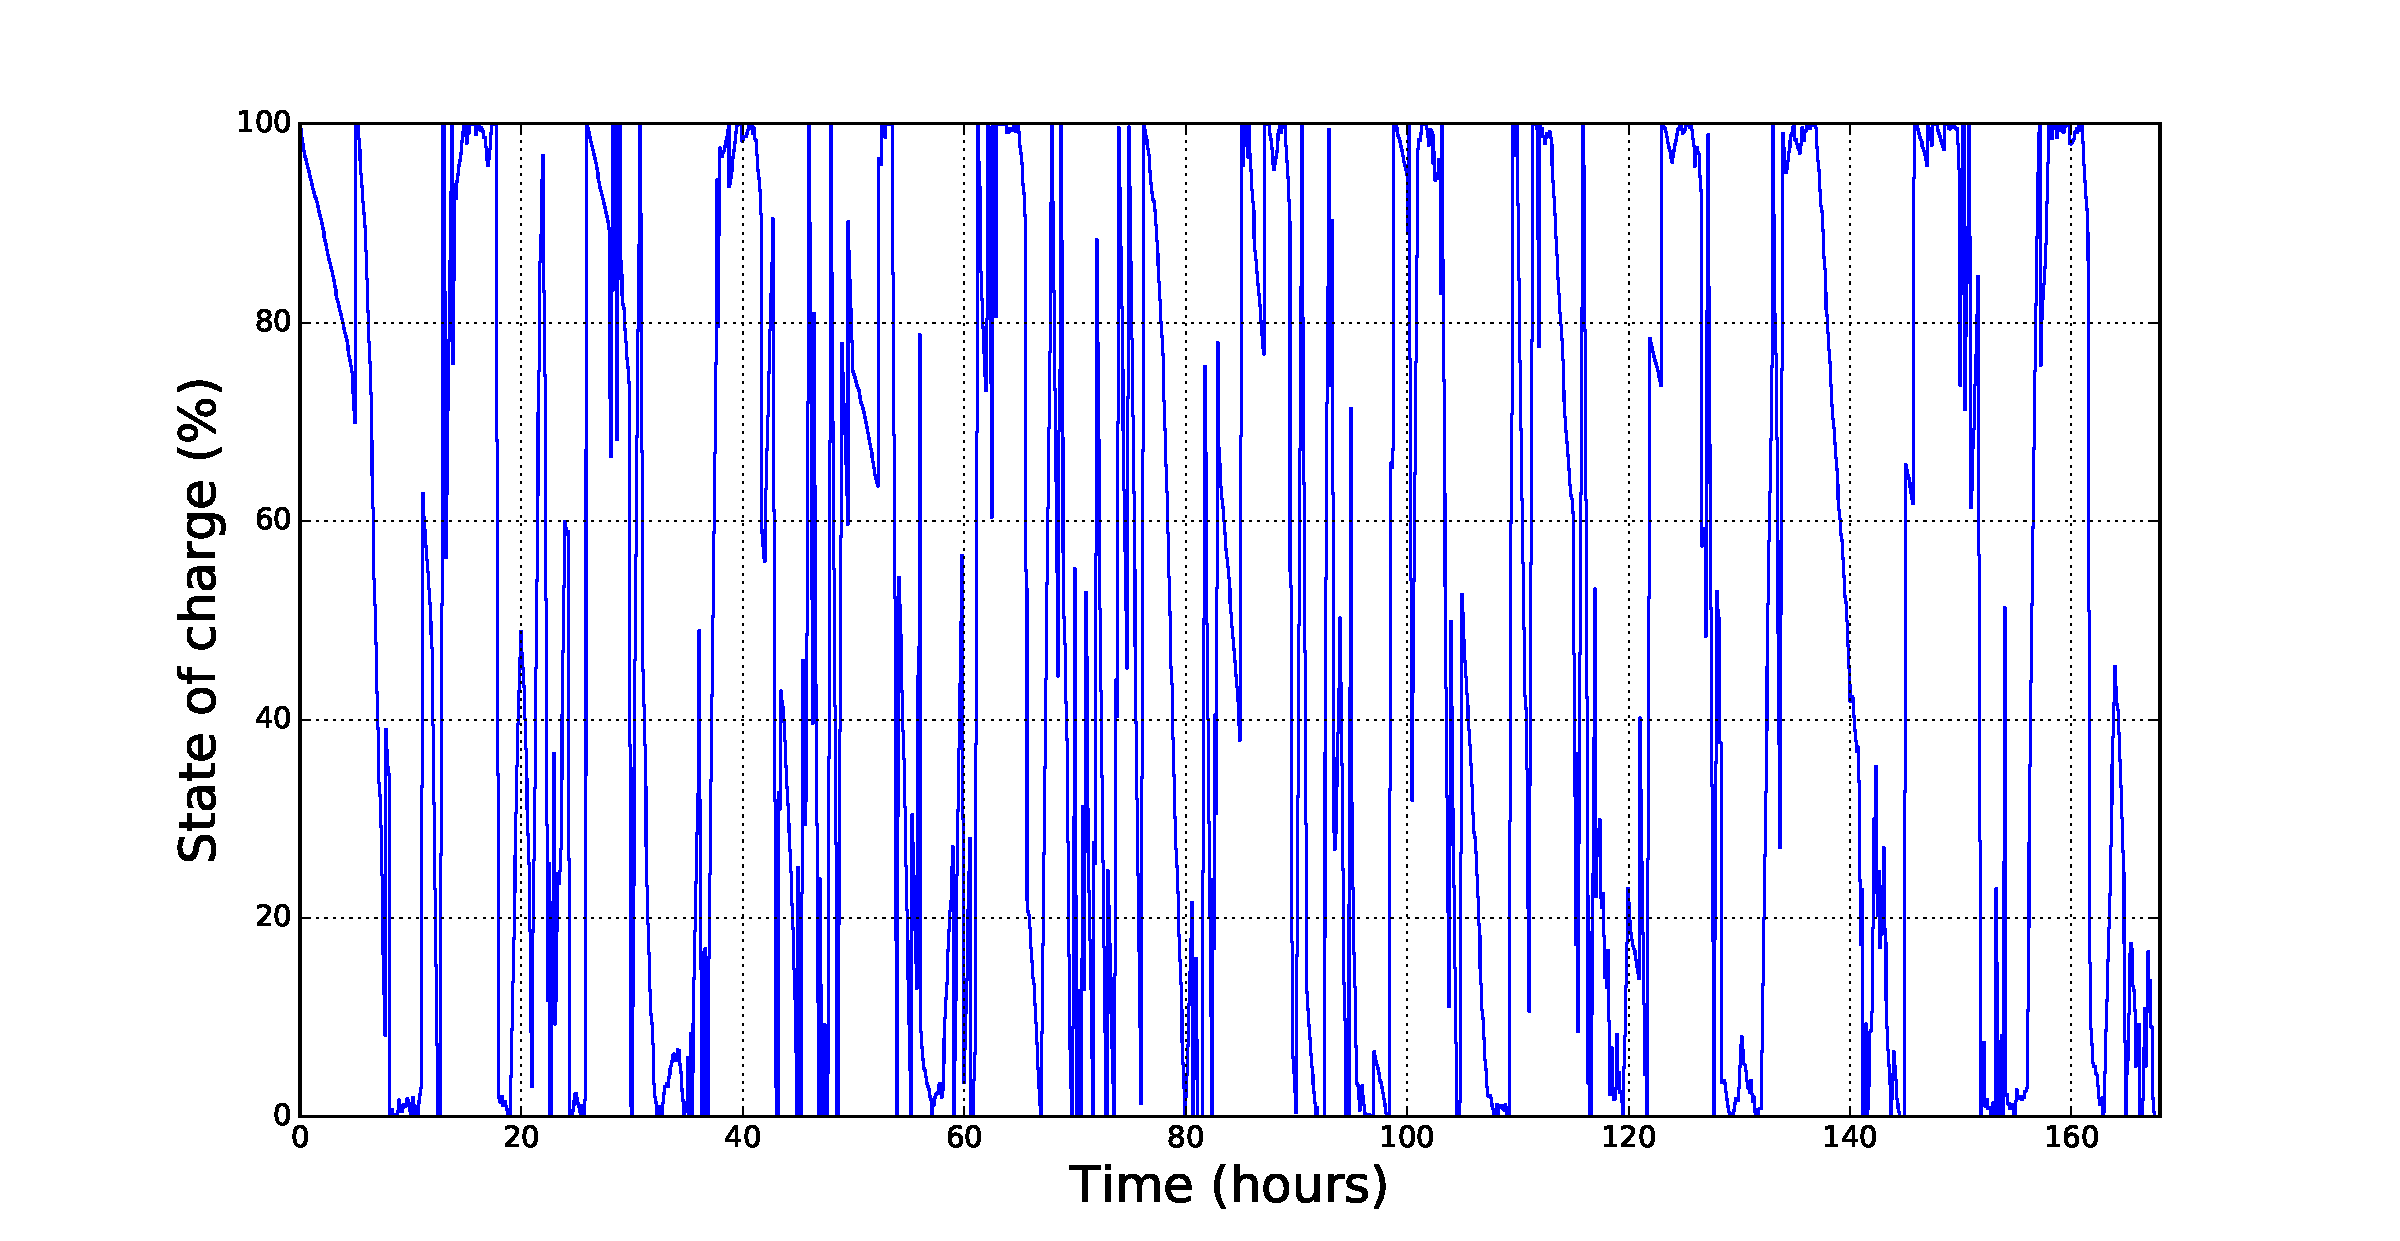
\includegraphics[width=\linewidth]{Figures/Plots/fullproblem_stoch/soc_fp_st.pdf} \caption{State of charge trajectory}\label{fig:soc_fp_st}
\end{subfigure}
\caption{Operating condition of battery when participating in both day-ahead and real-time markets}
\end{figure}
\FloatBarrier
\begin{figure}[h!]
\begin{center}
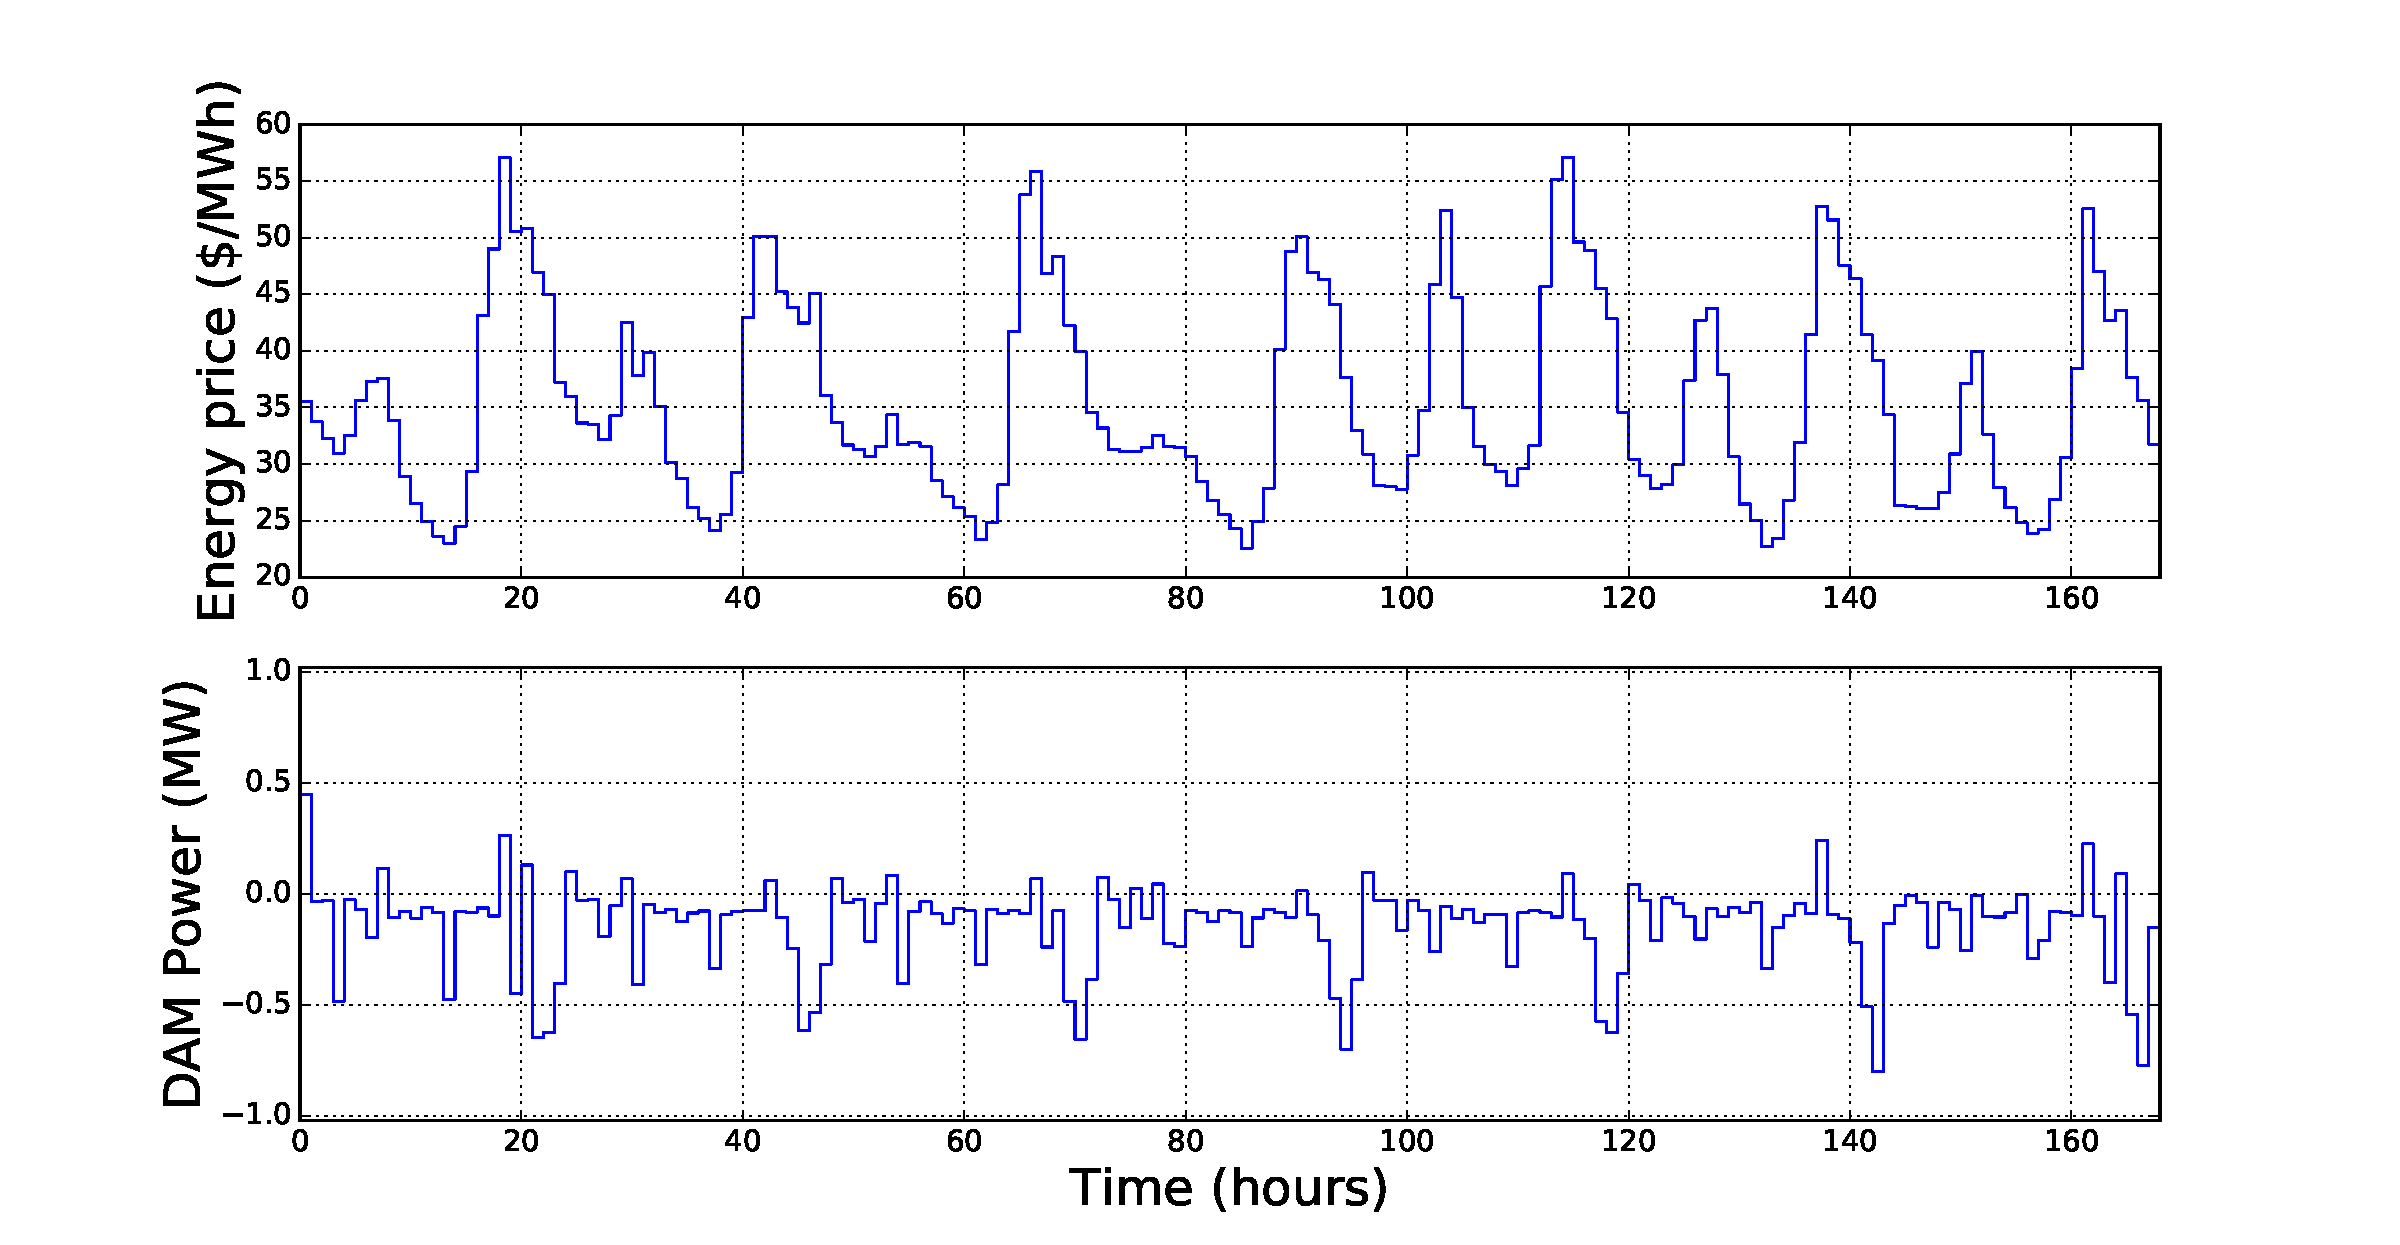
\includegraphics[width=4in]
{Figures/Plots/onlydam/Pdam_fp_st.pdf} \caption{Energy participation policy when battery participates only in day-ahead market.}\label{fig:Pdam_onlydam}\end{center}
\end{figure}
\begin{figure}[h!]
\begin{center}
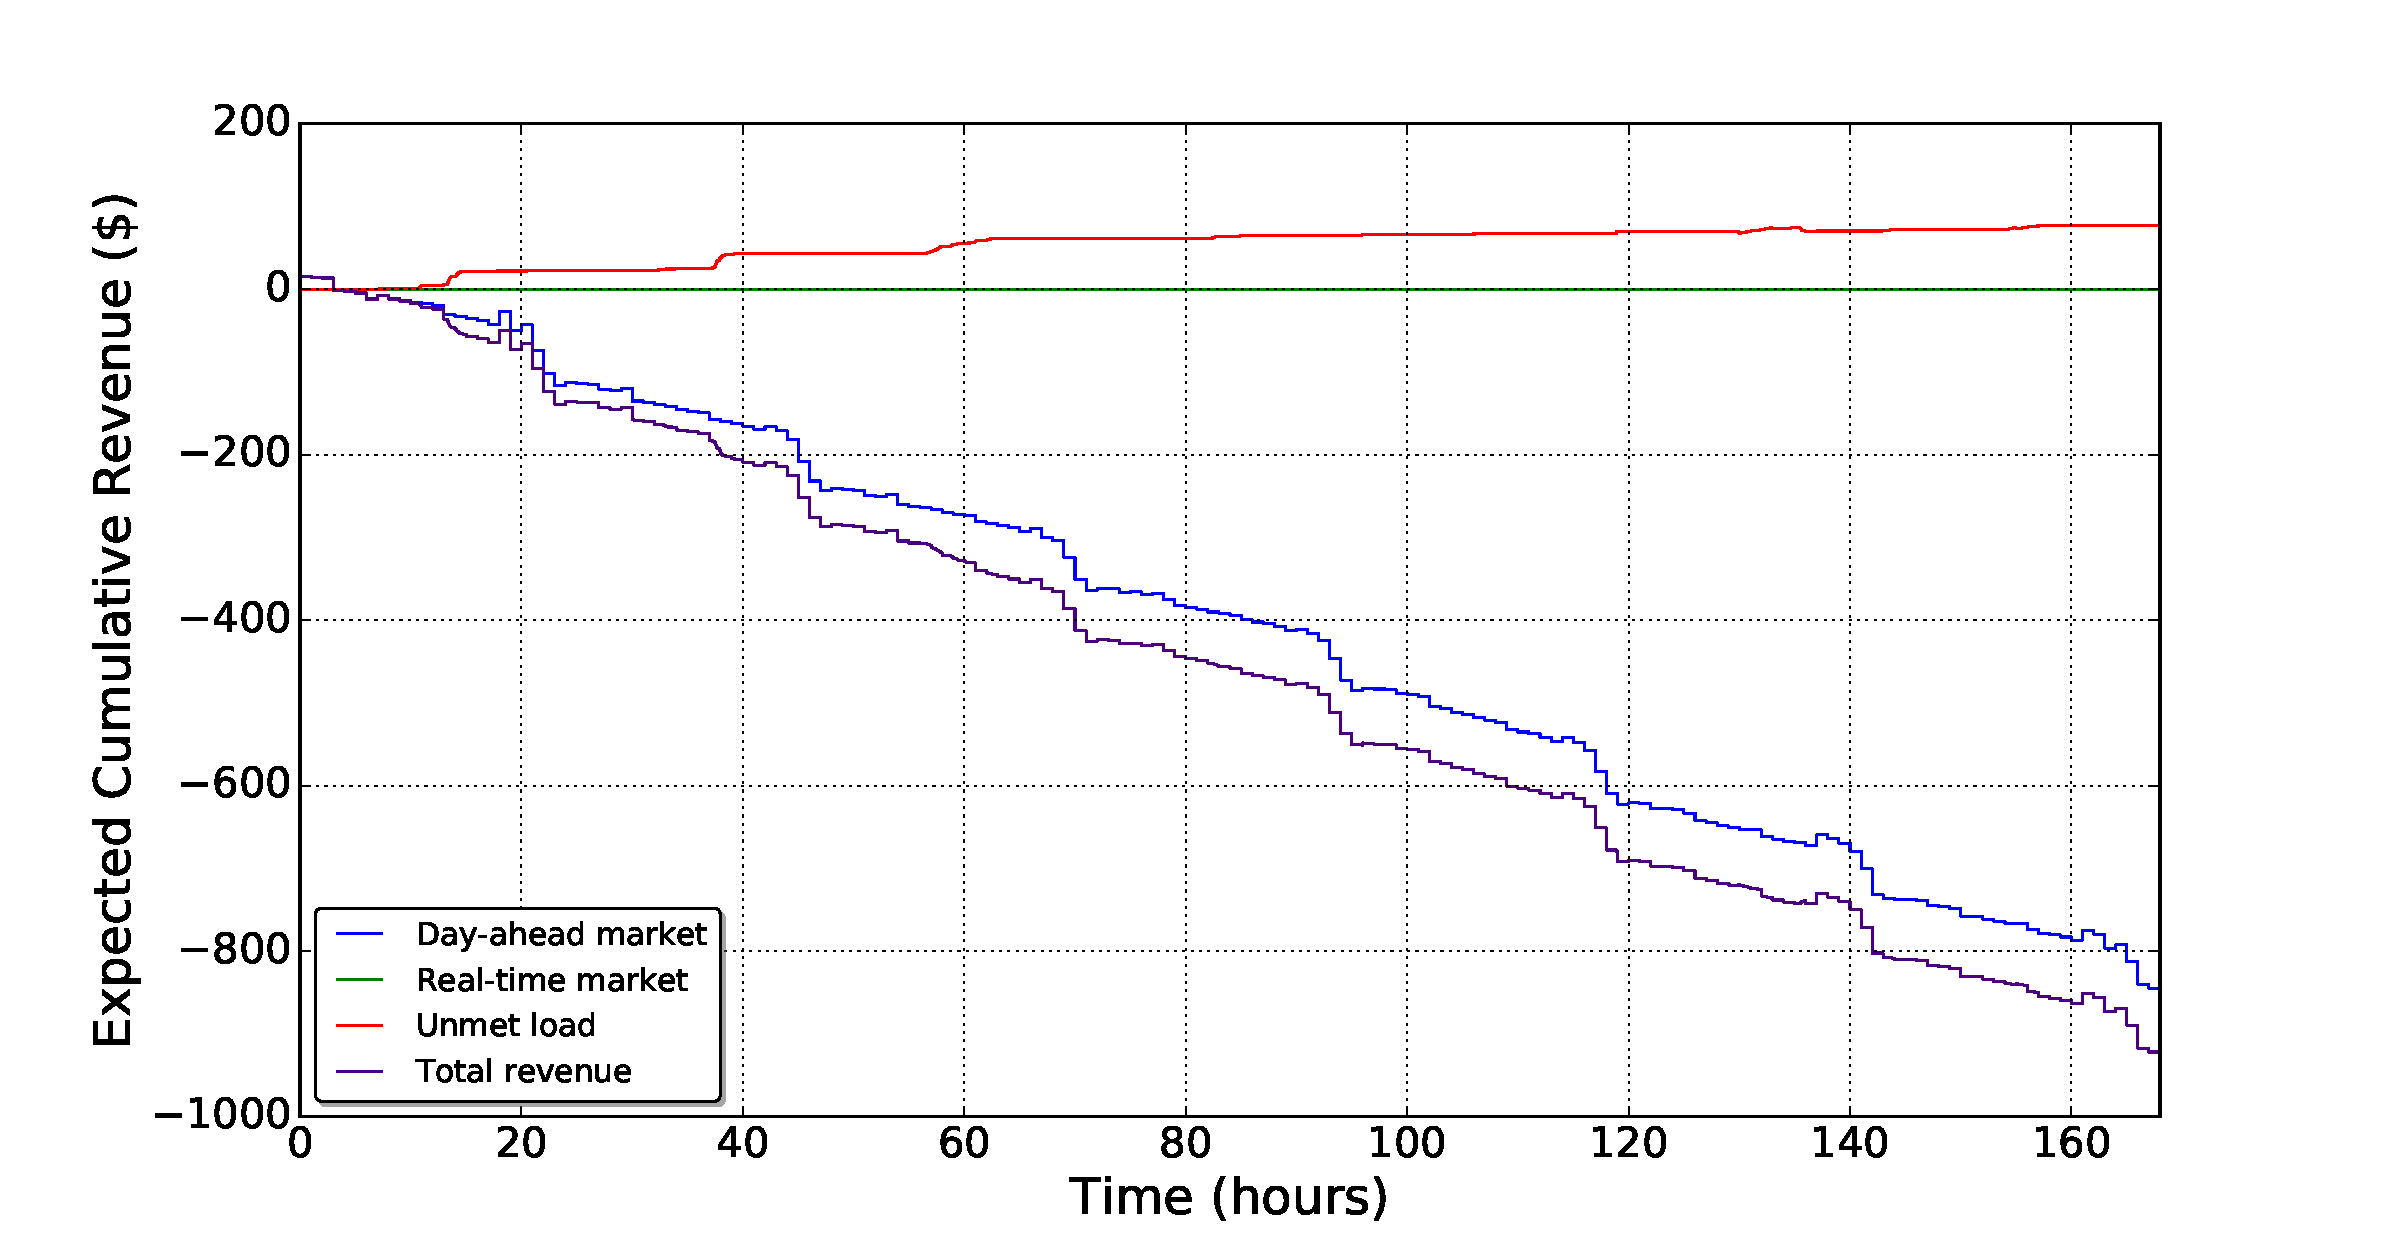
\includegraphics[width=4in]
{Figures/Plots/onlydam/cumulative_rev_fp_st.pdf} \caption{Trajectory of cumulative revenue when battery participates only in day-ahead market}\label{fig:cumulative_rev_onlydam}\end{center}
\end{figure}


\subsubsection{Upper Bound from Mean Value Problem}
total cost: -697.61

\subsubsection{Estimating Bounds with Perfect Information}
expected cost: -714.18 better than -711

\subsubsection{Estimating Bounds with Two-Stage Approximation: Restriction}
expected cost: -698.92
\subsection{Stochastic Dual Dynamic Programming}
final lower bound : -554.88
final upper bound : -554.79 confidence interval: [-554.57, -555.02]
time : 825.8 sec
\begin{figure}[h!]
\begin{center}
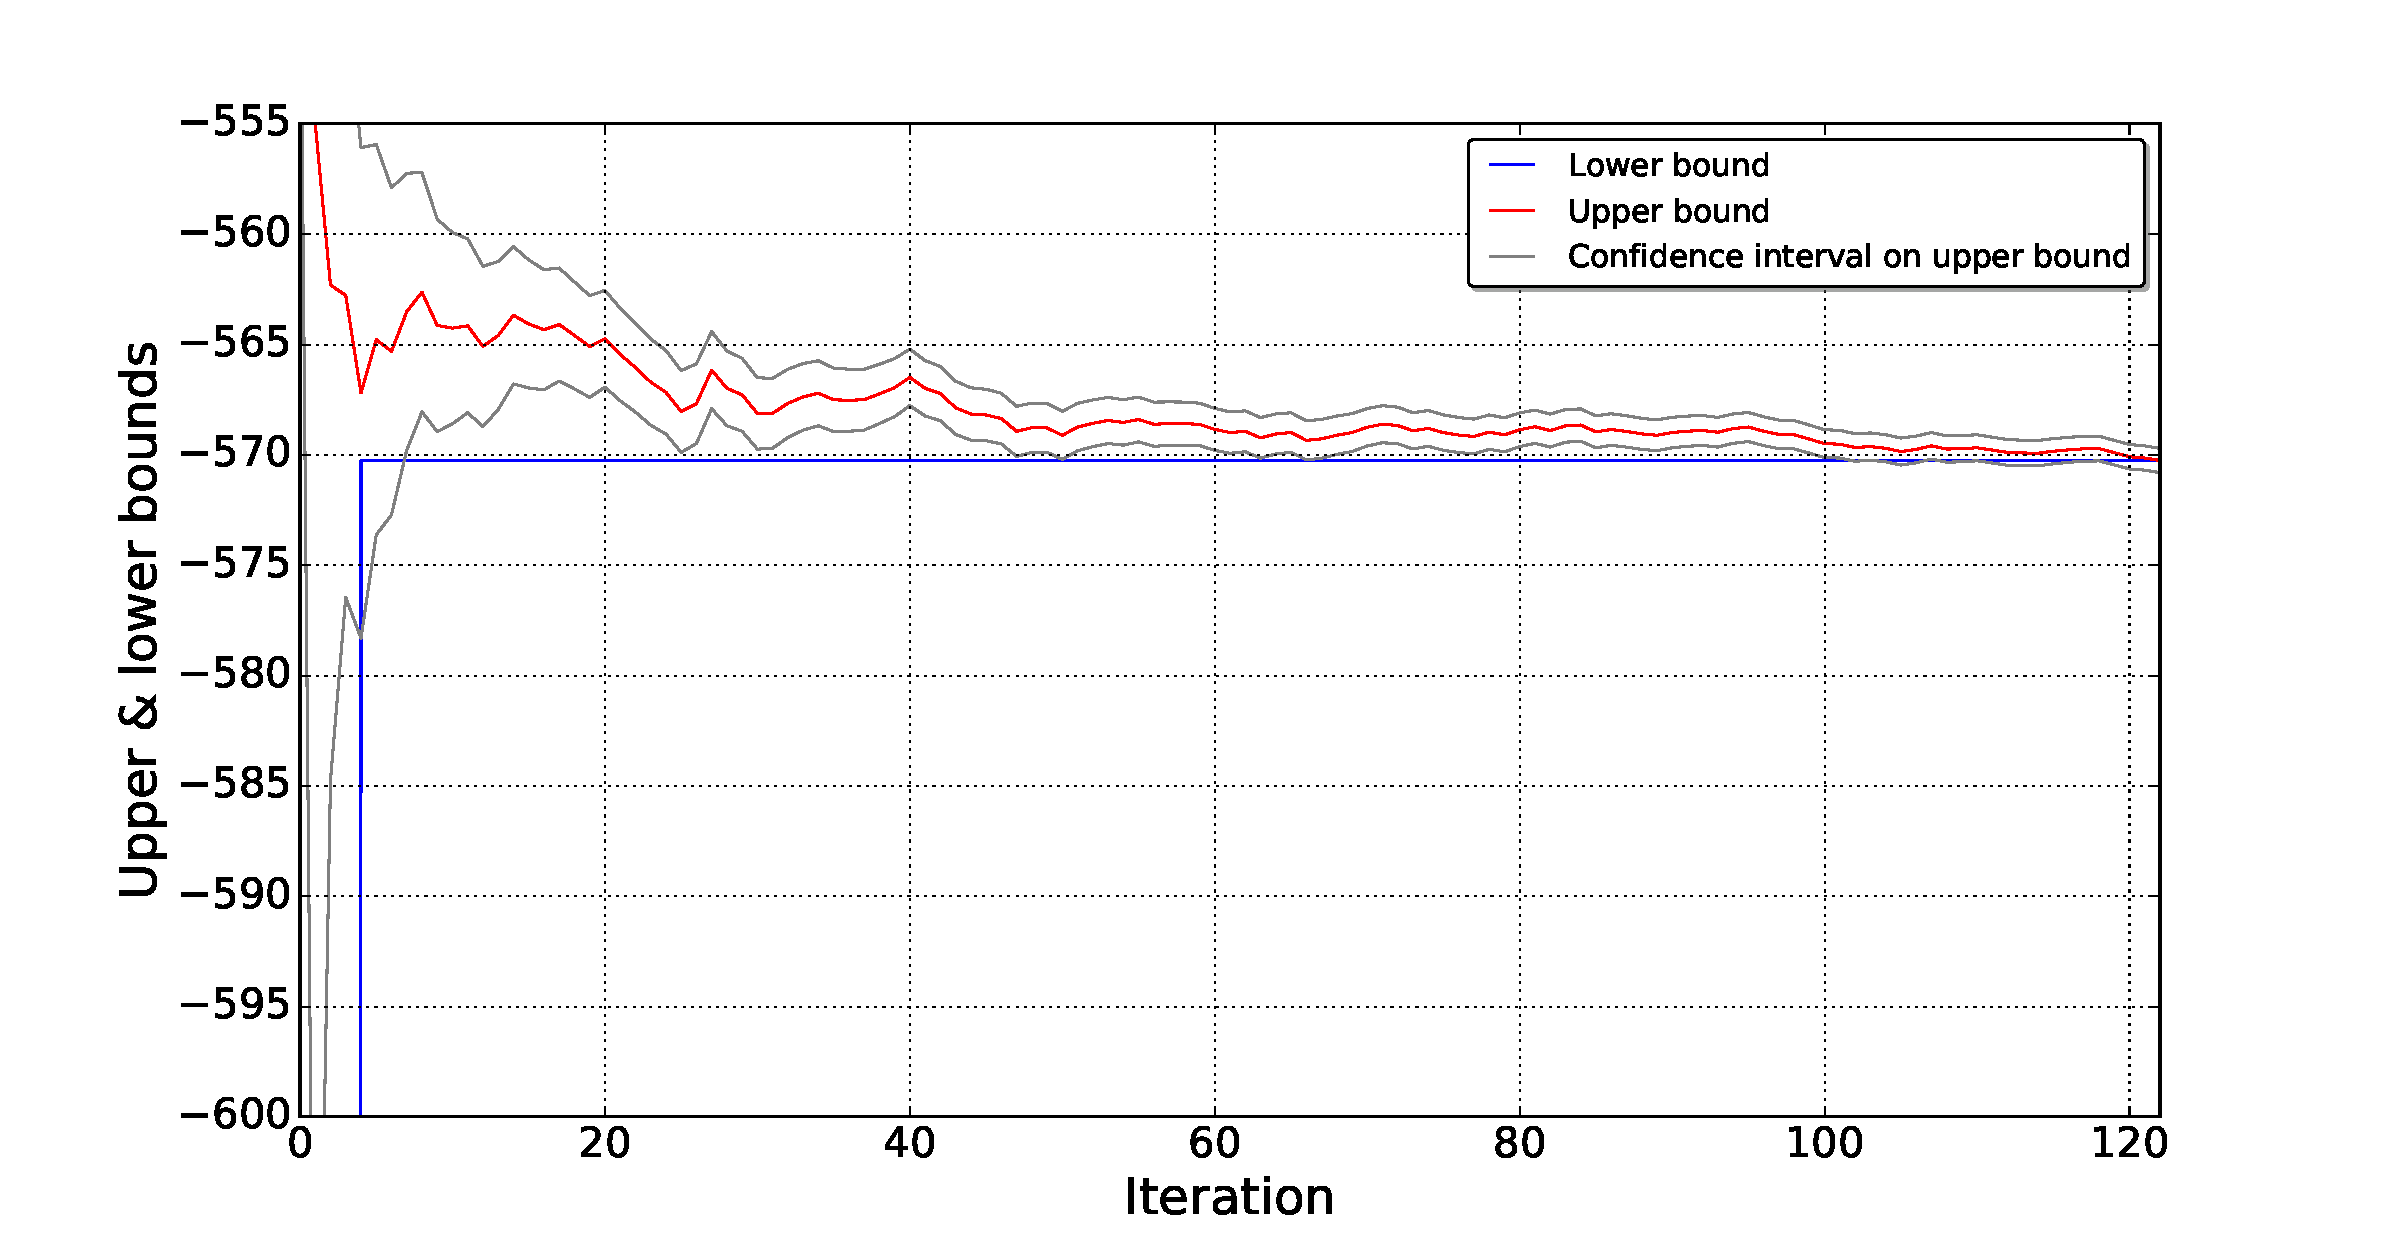
\includegraphics[scale=0.4]
{Figures/Plots/dualdynamic/bounds.pdf} \caption{Trajectory of the lowerand upper bounds obtained at every iteration of stochastic dual dynamic programming}\label{fig:bounds}\end{center}
\end{figure}

\FloatBarrier
\subsection{Receding Horizon Heuristic}
In practical situations, we may not have the sample scenarios for load profiles available for full week or a longer planning period that we want to schedule our market participation policy for. In situations when we have the profiles for load scenarios are available for less time periods, a receding horizon scheme is useful and can be implemented to minimize the cost looking at only that much ahead in future for which we have the sample load scenarios. The receding horizon scheme is expected to do worse than the case when we have sample scenarios for load profiles available for the full planning period, but it still outperforms a policy obtained using mean-value counterpart in the same situation (when we have information available for less period of time in future). 

We assume that at every hour $\tau$, we have a set of samples for the scenarios for load profiles available only for the next $T$ hours while we want to plan for a period $T_{P}$. At $\tau$, we can solve a stochastic program $\mathcal{P}_{\tau}$, where $\mathcal{P}_{\tau}$ is the extensive form of the stochastic program described in Section \ref{subsec:opt_unc} with $n_\text{dam} = T$. To solve this stochastic program, it requires the inputs $L_{i,k,s}$, $\pi_{i,k}$ and $\pi_k$ $\forall i \in \mathcal{T_R}, k \in \{\tau+1, ..., \tau+T\}, s \in \mathcal{S}$ and the initial energy level of the battery at that hour $\tau$, $E_{\tau}$. For compact representation, let $L_{\tau}(\xi_{\tau})$ denote the set of load profiles in all scenarios for future $T$ hours and $\pi_{\tau}$ be the set of prices in day-ahead and real-time markets for hour $\tau+1$ to $\tau+T$. We can now solve the $T$-hour horizon stoachastic program $\mathcal{P}_{\tau}\left(E_{\tau}, \pi_{\tau}, L_{\tau}(\xi_{\tau})\right)$.

The receding horizon scheme which we implement on the building-battery system is described below.
\begin{enumerate}
\item Consider $\tau = 0$.
\item With $E_\tau$, $L_{\tau}(\xi_{\tau})$ and $\pi_{\tau}$, solve the stochastic program $\mathcal{P}_{\tau}\left(E_{\tau}, \pi_{\tau}, L_{\tau}(\xi_{\tau})\right)$ over a $T$-hour horizon.
\item By solving $\mathcal{P}_{\tau}\left(E_{\tau}, \pi_{\tau}, L_{\tau}(\xi_{\tau})\right)$, obtain a profile for net battery discharge, $P_{net}$, between hours $\tau$ and $\tau+1$ corresponding to each scenario of load profile in the interval.
\item Using a realized scenario for load (random) between hours $\tau$ and $\tau+1$, evolve battery storage level to $E_{\tau+1}$.
\item Set $\tau = \tau+1$.
\item If $\tau = T_P$, then stop, else go to step 2.
\end{enumerate}




We sample 50 paths upto next 24 hours horizon
\section{Conclusions}
Expected objective over 100 runs for stochastic fullproblem = -712.9901530720865
Confidence interval on objective over 100 runs = (-713.3345792874304,-712.6457268567426)

\section{Future Work}

\subsection{Price Uncertainty}

\subsection{Three Layer Markets}



\bibliography{cs719}

\end{document}
